%===============================================================================
% LaTeX sjabloon voor de bachelorproef toegepaste informatica aan HOGENT
% Meer info op https://github.com/HoGentTIN/latex-hogent-report
%===============================================================================

\documentclass[dutch,dit,thesis]{hogentreport}

\usepackage{lipsum}
\usepackage{pgfgantt}
\usepackage{tabularx}
\usepackage{graphicx}
\usepackage{csquotes}
\usepackage{multicol}
\usepackage{listings}

% \setquotestyle{english}
\DeclareQuoteStyle{house}
    {\textquotedblleft}{\textquotedblright}
    {\textquoteleft}{\textquoteright}

%% Pictures to include in the text can be put in the graphics/ folder
\graphicspath{{graphics/}}

%% For source code highlighting, requires pygments to be installed
%% Compile with the -shell-escape flag!
\usepackage[section]{minted}
\usemintedstyle{solarized-light}
\definecolor{bg}{RGB}{253,246,227} %% Set the background color of the codeframe

%% Change this line to edit the line numbering style:
\renewcommand{\theFancyVerbLine}{\ttfamily\scriptsize\arabic{FancyVerbLine}}

%% Macro definition to load external java source files with \javacode{filename}:
\newmintedfile[javacode]{java}{
    bgcolor=bg,
    fontfamily=tt,
    linenos=true,
    numberblanklines=true,
    numbersep=5pt,
    gobble=0,
    framesep=2mm,
    funcnamehighlighting=true,
    tabsize=4,
    obeytabs=false,
    breaklines=true,
    mathescape=false
    samepage=false,
    showspaces=false,
    showtabs =false,
    texcl=false,
}

% Other packages not already included can be imported here
\usepackage{xcolor}
\newcommand\ytl[2]{
    \parbox[b]{8em}{\hfill{\color{cyan}\bfseries\sffamily #1}~$\cdots\cdots$~}\makebox[0pt][c]{$\bullet$}\vrule\quad \parbox[c]{13cm}{\vspace{12pt}\color{red!40!black!80}\raggedright\sffamily #2.\\[7pt]}\\[-3pt]}


%%---------- Document metadata -------------------------------------------------
\author{Dylan Vermeersch}
\supervisor{Dhr. L. Blondeel}
\cosupervisor{Dhr. D. Marichal}
\title{Onderzoek naar de compilatie en bind van een Coolgen programma via een Azure DevOps pipeline binnen de mainframe omgeving van ArcelorMittal Gent met proof of concept.}
\academicyear{\advance\year by -1 \the\year--\advance\year by 1 \the\year}
\examperiod{1}
\degreesought{\IfLanguageName{dutch}{Professionele bachelor in de toegepaste informatica}{Bachelor of applied computer science}}
\partialthesis{false}

%% Add global exceptions to the hyphenation here
\hyphenation{back-slash}

%% The bibliography (style and settings are  found in hogentthesis.cls)
\addbibresource{bachproef.bib}            %% Bibliography file
\addbibresource{../voorstel/voorstel.bib} %% Bibliography research proposal
\defbibheading{bibempty}{}

%% Prevent empty pages for right-handed chapter starts in twoside mode
\renewcommand{\cleardoublepage}{\clearpage}

\renewcommand{\arraystretch}{1.2}

%% Content starts here.
\begin{document}

%---------- Front matter -------------------------------------------------------

\frontmatter

\hypersetup{pageanchor=false} %% Disable page numbering references
%% Render a Dutch outer title page if the main language is English
\IfLanguageName{english}{%
    %% If necessary, information can be changed here
    \degreesought{Professionele Bachelor toegepaste informatica}%
    \begin{otherlanguage}{dutch}%
       \maketitle%
    \end{otherlanguage}%
}{}

%% Generates title page content
\maketitle
\hypersetup{pageanchor=true}

%%=============================================================================
%% Voorwoord
%%=============================================================================

\chapter*{\IfLanguageName{dutch}{Woord vooraf}{Preface}}%
\label{ch:voorwoord}

Voor u ligt mijn bachelorproef getiteld \enquote{Onderzoek naar de compilatie en bind van een Coolgen programma via een Azure DevOps pipeline binnen de mainframe omgeving van ArcelorMittal Gent met proof of concept}. 
Deze bachelorproef is geschreven als een vereiste voor het behalen van mijn afstudeerdiploma in de richting \enquote{Toegepaste Informatica} aan HoGent.
Gedurende de periode van februari tot mei 2024 heb ik me beziggehouden met het onderzoeken en het schrijven van deze bachelorproef. 
\\ \\
Gedurende mijn tijd aan HoGent heb ik lang getwijfeld waar ik later mijn job van wou maken, er was niets dat mijn interesse voor de volle 100\% kon wekken. 
Dit allemaal veranderde toen er op het einde van mijn tweede jaar in de opleiding Toegepaste Informatica de term mainframe naar mijn hoofd werd geslingerd. 
Ik was meteen heel erg geïnteresseerd in deze nieuwe term en vroeg mijn medestudenten Muhammed en Mehmet om meer informatie over het onderwerp. 
Het bleek al snel dat het een hot topic was binnen de wereld van big IT, we hebben toen ook de vraag gesteld aan Dhr. Leendert Blondeel of het mogelijk was om meer duiding te geven bij de specialisatierichting Mainframe Expert. 
Dit verzoek werd met veel enthousiasme onthaald en vrijwel meteen werd een virtueel gesprek ingepland met mijzelf, Mehmet en Muhammed om ons meer te vertellen over mainframe en hoe een jaar van een mainframe student op HoGent eruitziet.
Meteen tijdens het gesprek wist ik dat ik mijn afstudeerrichting gevonden had, de passie was en is nog altijd heel erg groot bij Dhr. Leendert Blondeel en trok je direct aan zoals normaal alleen een magneet dat kan. 
\\ \\
Het werd tijdens dat derde jaar alleen maar duidelijker dat ik de juiste weg ingeslagen was, we ontmoetten enorm veel mensen die net zoals Dhr. Leendert Blondeel heel erg gepassioneerd zijn over mainframe en alles daaromtrent. 
Veel van deze mensen zijn nog altijd goed bereikbaar via mail ondanks het feit dat ze bij heel grote bedrijven zitten, kan ik ze nog altijd bereiken voor allerhande vragen over bijeenkomsten, mainframe topics of zelfs om de ondervindingen van mijn bachelorproef mee te delen. 
Het heeft me duidelijk geen windeieren gelegd om de keuze voor mainframe te maken. 
\\ \\
Graag wil ik mijn begeleider, Dhr. Leendert Blondeel, bedanken voor zijn uitstekende begeleiding en ondersteuning gedurende dit onderzoek. 
Zijn begeleiding heeft mijn leermogelijkheden gemaximaliseerd, waarvoor ik hem zeer dankbaar ben. 
Ook wil ik Dhr. Didier Marichal van ArcelorMittal Gent bedanken voor zijn bijdrage aan dit onderzoek als co-promotor. 
\\ \\
Tot slot wil ik ook het mainframe systeembeheer team van ArcelorMittal Gent bedanken, ik kon elk moment van de dag bij hun terecht met allerhande vragen of zelfs om een gezellig babbeltje te slaan. 
Ze zorgden ervoor dat ik me heel erg thuis voelde binnen het team. 
Graag wil ik ook nog mijn familie en vrienden bedanken voor hun steun gedurende mijn onderzoeksproces. 
\\ \\
Ik wens u veel leesplezier.
\\ \\
Dylan Vermeersch
\\
Oostakker, 24 mei 2024
%%=============================================================================
%% Samenvatting
%%=============================================================================

% TODO: De "abstract" of samenvatting is een kernachtige (~ 1 blz. voor een
% thesis) synthese van het document.
%
% Een goede abstract biedt een kernachtig antwoord op volgende vragen:
%
% 1. Waarover gaat de bachelorproef?
% 2. Waarom heb je er over geschreven?
% 3. Hoe heb je het onderzoek uitgevoerd?
% 4. Wat waren de resultaten? Wat blijkt uit je onderzoek?
% 5. Wat betekenen je resultaten? Wat is de relevantie voor het werkveld?
%
% Daarom bestaat een abstract uit volgende componenten:
%
% - inleiding + kaderen thema
% - probleemstelling
% - (centrale) onderzoeksvraag
% - onderzoeksdoelstelling
% - methodologie
% - resultaten (beperk tot de belangrijkste, relevant voor de onderzoeksvraag)
% - conclusies, aanbevelingen, beperkingen
%
% LET OP! Een samenvatting is GEEN voorwoord!

%%---------- Nederlandse samenvatting -----------------------------------------
%
% TODO: Als je je bachelorproef in het Engels schrijft, moet je eerst een
% Nederlandse samenvatting invoegen. Haal daarvoor onderstaande code uit
% commentaar.
% Wie zijn bachelorproef in het Nederlands schrijft, kan dit negeren, de inhoud
% wordt niet in het document ingevoegd.

\IfLanguageName{english}{%
\selectlanguage{dutch}
\chapter*{Samenvatting}
\lipsum[1-4]
\selectlanguage{english}
}{}

%%---------- Samenvatting -----------------------------------------------------
% De samenvatting in de hoofdtaal van het document

\chapter*{\IfLanguageName{dutch}{Samenvatting}{Abstract}}

\lipsum[1-4]


%---------- Inhoud, lijst figuren, ... -----------------------------------------

\tableofcontents

% In a list of figures, the complete caption will be included. To prevent this,
% ALWAYS add a short description in the caption!
%
%  \caption[short description]{elaborate description}
%
% If you do, only the short description will be used in the list of figures

\listoffigures

% If you included tables and/or source code listings, uncomment the appropriate
% lines.
%\listoftables
%\listoflistings

% Als je een lijst van afkortingen of termen wil toevoegen, dan hoort die
% hier thuis. Gebruik bijvoorbeeld de ``glossaries'' package.
% https://www.overleaf.com/learn/latex/Glossaries

%---------- Kern ---------------------------------------------------------------

\mainmatter{}

% De eerste hoofdstukken van een bachelorproef zijn meestal een inleiding op
% het onderwerp, literatuurstudie en verantwoording methodologie.
% Aarzel niet om een meer beschrijvende titel aan deze hoofdstukken te geven of
% om bijvoorbeeld de inleiding en/of stand van zaken over meerdere hoofdstukken
% te verspreiden!

%%=============================================================================
%% Inleiding
%%=============================================================================

\chapter{\IfLanguageName{dutch}{Inleiding}{Introduction}}%
\label{ch:inleiding}

Deze bachelorproef gaat over op welke manier er een Azure DevOps pipeline kan geïntegreerd worden binnen ArcelorMittal Gent om hun bestaande en toekomstige Coolgen programma's te compilen/binden. 
Dit onderzoek is begonnen omdat ArcelorMittal Gent graag hun mainframe omgeving wil moderniseren en automatiseren, meer bepaald gaat het in dit onderzoek over het automatiseren van de compile/bind van Coolgen programma's.



\section{\IfLanguageName{dutch}{Probleemstelling}{Problem Statement}}%
\label{sec:probleemstelling}

Bij ArcelorMittal Gent wordt er gekeken hoe men hun mainframe omgeving kan moderniseren, op die manier kunnen ze efficiënt gebruik maken van de nieuwe technologieën die de laatste jaren in opmars zijn zoals automatische DevOps pipelines. 
Door zaken zoals het compileren/binden van programma's automatisch te starten via een pipeline wordt er aan tijd gewonnen wat er dus voor zorgt dat een taak efficiënter wordt. 
Bij ArcelorMittal Gent zijn ze daarom op zoek naar een manier om het compile/bind proces voor hun Coolgen programma's te automatiseren met behulp van een Azure DevOps pipeline.
Momenteel is het nog niet duidelijk wat ervoor nodig is om zo'n Azure DevOps pipeline werkende te krijgen voor bestaande en toekomstige Coolgen programma's binnen ArcelorMittal Gent.

\section{\IfLanguageName{dutch}{Onderzoeksvraag}{Research question}}%
\label{sec:onderzoeksvraag}

Op welke manier kan er een Azure DevOps pipeline geïntegreerd worden om de compile/bind van bestaande en toekomstige Coolgen programma's uit te voeren. 
Wat zijn de gevolgen voor het huidige compile/bind systeem voor Coolgen programma's na het integreren van de bekomen pipeline met de mainframe omgeving van ArcelorMittal Gent. 

\section{\IfLanguageName{dutch}{Onderzoeksdoelstelling}{Research objective}}%
\label{sec:onderzoeksdoelstelling}

Het onderzoek moet een duidelijk beeld geven over welke technologieën er gebruikt worden om een Azure DevOps pipeline op te zetten die als taak heeft om de compile/bind van Coolgen programma's te verzorgen.
Een proof of concept wordt opgesteld om zo'n Azure DevOps pipeline uit te werken die de compile/bind van bestaande en toekomstige Coolgen programma's kan uitvoeren. 

\section{\IfLanguageName{dutch}{Opzet van deze bachelorproef}{Structure of this bachelor thesis}}%
\label{sec:opzet-bachelorproef}
De rest van deze bachelorproef is als volgt opgebouwd:

In Hoofdstuk~\ref{ch:stand-van-zaken} wordt een overzicht gegeven van de stand van zaken binnen het onderzoeksdomein, op basis van een literatuurstudie.

In Hoofdstuk~\ref{ch:methodologie} wordt de methodologie toegelicht en worden de gebruikte onderzoekstechnieken besproken om een antwoord te kunnen formuleren op de onderzoeksvragen.

In Hoofdstuk~\ref{ch:current system} wordt de werking van het huidige systeem in verband met de compilatie en bind van een programma toegelicht. 

In Hoofdstuk~\ref{ch:poc} wordt de uitvoering van de Proof Of Concept toegelicht en welke aanpassingen moesten gebeuren aan het product DBB van IBM. 

In Hoofdstuk~\ref{ch:conclusie}, tenslotte, wordt de conclusie gegeven en een antwoord geformuleerd op de onderzoeksvragen. Daarbij wordt ook een aanzet gegeven voor toekomstig onderzoek binnen dit domein.
\chapter{\IfLanguageName{dutch}{Stand van zaken}{State of the art}}%
\label{ch:stand-van-zaken}

% Tip: Begin elk hoofdstuk met een paragraaf inleiding die beschrijft hoe
% dit hoofdstuk past binnen het geheel van de bachelorproef. Geef in het
% bijzonder aan wat de link is met het vorige en volgende hoofdstuk.

% Pas na deze inleidende paragraaf komt de eerste sectiehoofding.

% Let er ook op: het \texttt{cite}-commando voor de punt, dus binnen de zin. Je verwijst meteen naar een bron % in de eerste zin die erop gebaseerd is, dus niet pas op het einde van een paragraaf.

In de snel evoluerende wereld van technologie speelt de mainframe nog altijd een essentiële rol als krachtige en betrouwbare computerinfrastructuur. Het is de ruggengraat van talloze organisaties, variërend van grote bedrijven tot overheidsinstanties, die vertrouwen op mainframes voor het verwerken van bedrijfskritieke workloads. Met de opkomst van moderne applicatie-ontwikkeling en de behoefte aan automatisering van het software ontwikkelproces, hebben mainframes zich aangepast aan het veranderende landschap. Dit doen ze door het aanbieden van de DevOps werkwijze en geavanceerde technologieën zoals Git, Azure DevOps en IBM Dependency Based Build ook wel bekend als IBM DBB.
\\ \\
Deze literatuurstudie onderzoekt de samenstelling van mainframe-technologie, IBM Dependency Based Build, Azure DevOps en Git workflows als een krachtige combinatie om een brug te slaan tussen het legendarische mainframe-erfgoed en het moderne automatisatie-gedreven software ontwikkelproces. Het onderzoek verkent de essentie van mainframes en hun evolutie door de jaren heen, evenals de cruciale rol die ze blijven spelen in het ondersteunen van kritieke bedrijfsprocessen.
\\ \\
Daarnaast wordt er dieper ingegaan op IBM Dependency Based Build, een krachtige tool ontwikkeld door IBM om mainframes te verbinden met moderne DevOps tools zoals Azure DevOps en Git. De studie onderzoekt de kenmerken en voordelen van IBM DBB en hoe dat het mogelijk maakt om een mainframe landschap open te stellen tot de DevOps werkwijze om op die manier software te ontwikkelen op de wijze waarop veel moderne platformen dat ook doen.
\\ \\
Verder wordt de focus gelegd op Azure DevOps, een krachtige tool-set die onder andere Azure Repos en Azure Pipelines bevat. Beide zijn noodzakelijk voor een goede DevOps werkwijze op te zetten. De studie verkent de mogelijkheden van de tool-set, zoals de verschillende onderdelen ervan en hoe deze bijdragen aan een DevOps werkomgeving.
\\ \\
Tot slot komt ook Git workflows aan bod, dit is een manier van werken om zo de flow van het software ontwikkelproces te bepalen. Dit is noodzakelijk voor de integriteit van de software die ontwikkeld wordt te bewaren. Er wordt in de studie onderzoekt wat een Git workflow is, welke workflow het best aanleunt tegen de mainframe waarden die zo hoog aangeschreven staan zoals betrouwbaarheid, integriteit en veiligheid.
\\ \\
\section{De mainframe}
\label{sec:de mainframe}

\subsection{Etymologie van de term mainframe}
De term mainframe is afgeleid van het Engelse woord ”frame”, dat in dit geval verwijst naar de behuizing of structuur van de computer. Het woord ”main” duidt op de centrale rol van deze computer in een gegevensverwerkingsomgeving. Een mainframe was bedoeld als het belangrijkste systeem in een computerinstallatie, waar andere randapparatuur en terminals op waren aangesloten \autocite{IBM2024}.
\\ \\
De oorsprong van de term mainframe kan worden toegeschreven aan de evolutie van computersystemen van die tijd. In de beginjaren van computers werden ze meestal aangeduid als grote computers of elektronische rekenmachines. Naarmate de technologie vorderde en de computers krachtiger en complexer werden, ontstond de behoefte aan een specifieke term om deze geavanceerde systemen te beschrijven \autocite{IBM2024}.
\\ \\
\subsection{Historie van de IBM mainframe}
De IBM mainframe heeft een rijke geschiedenis die teruggaat tot de vroege dagen van de computertechnologie.
\\ \\
\subsubsection{IBM 701 Electronic Data Processing machine (1952)}
In 1952 werd de IBM 701 gelanceerd als een geavanceerde elektronische gegevensverwerkingsmachine. Het was ontworpen om wetenschappelijke berekeningen en gegevensverwerkingstaken uit te voeren en bood meer rekenkracht en geheugencapaciteit dan eerdere computersystemen aan \autocite{IBM2024a}.
\\ \\
De IBM 701 maakte gebruik van vacuümbuizen als belangrijkste elektronische componenten en kon ongeveer 10.000 optellingen per seconde uitvoeren. Het systeem werd voornamelijk gebruikt door overheidsinstanties, laboratoria en grote bedrijven voor complexe wetenschappelijke en technische berekeningen \autocite{IBM2024a}.
\\ \\
De IBM 701 markeerde een belangrijke ontwikkeling in de computertechnologie, aangezien het een van de eerste commercieel succesvolle computers was die specifiek werd ontworpen voor gegevensverwerking. Het opende de deur naar geavanceerdere computersystemen en legde de basis voor toekomstige mainframes \auocite{IBM2024a}.
\\ \\
\subsubsection{IBM System/360 (1964)}
De ontwikkeling van de IBM/360 begon in de late jaren 1950 als een ambitieus project binnen IBM om een nieuwe generatie computersystemen te creëren die compatibiliteit zouden bieden tussen verschillende modellen. Het doel was om een reeks computers te ontwikkelen die zowel kleinere als grotere organisaties kon bedienen \autocite{IBM2024b}.
\\ \\
Op 7 april 1964 werd de IBM/360 officieel geïntroduceerd en werd het de eerste commercieel succesvolle mainframe computerreeks. Het systeem bood een breed scala aan modellen met verschillende prestatieniveaus en configuraties, waardoor het aan de behoeften van verschillende organisaties kon voldoen \autocite{IBM2024b}.
\\ \\
De IBM/360 was revolutionair omdat het een gemeenschappelijke architectuur introduceerde die compatibiliteit bood tussen de verschillende modellen. Hierdoor konden klanten hun investeringen in software en hardware beschermen, omdat programma’s op meerdere systemen konden draaien. Het was ook een van de eerste computersystemen die gebruikmaakte van geïntegreerde schakelingen \autocite{IBM2024b}.
\\ \\
De IBM/360 had een enorme impact op de computerindustrie en droeg bij aan de standaardisatie van computerarchitectuur. Het systeem werd breed geadopteerd door bedrijven, overheden en academische instellingen over de hele wereld en legde de basis voor latere ontwikkelingen in de mainframe-technologie \autocite{IBM2024b}.
\\ \\
\subsubsection{IBM System/370 (1970)}
De IBM/370 werd gelanceerd als opvolger van de IBM/360 en introduceerde belangrijke technologische verbeteringen, waaronder een uitgebreidere instructieset, verbeterde virtualisatiemogelijkheden en grotere geheugencapaciteit. Deze verbeteringen maakten het systeem krachtiger en veelzijdiger \autocite{IBM2024c}.
\\ \\
Een belangrijk kenmerk van de IBM/370 was de ondersteuning voor virtual memory, waardoor meerdere programma’s tegelijkertijd konden uitgevoerd worden en gebruik maken van het beschikbare geheugen. Dit leidde tot verbeterde systeemprestaties en efficiënter gebruik van resources \autocite{IBM2024c}.
\\ \\
De IBM/370 mainframe werd breed gebruikt door bedrijven en overheidsinstanties voor diverse toepassingen, waaronder gegevensverwerking, transactionele systemen, wetenschappelijke berekeningen en databasebeheer. Het bood hogere prestaties en schaalbaarheid, waardoor het kon voldoen aan de groeiende behoeften van organisaties \autocite{IBM2024c}.
\\ \\
\subsubsection{IBM System ZSeries (2000)}
De IBM zSeries, gelanceerd in het jaar 2000, was een belangrijke mijlpaal voor de mainframe-industrie. Het bood verschillende baanbrekende kenmerken en voordelen die een grote impact hadden.
\\ \\
Een van de belangrijkste aspecten van de zSeries was de aanzienlijke verbetering in prestaties en schaalbaarheid. Het systeem was in staat om enorme werklasten te verwerken en te voldoen aan de groeiende behoeften van bedrijven. Dit maakte het een krachtige keuze voor organisaties die behoefte hadden aan grote rekenkracht en verwerkingscapaciteit \autocite{IBM2024d}.
\\ \\
Naast prestatieverbeteringen stond de zSeries bekend om zijn ongeëvenaarde betrouwbaarheid en beschikbaarheid. Het bevatte geavanceerde functies zoals redundantie, fouttolerantie en hot-swappable componenten. Deze kenmerken minimaliseerden ongeplande downtime en waarborgden een hoge beschikbaarheid van systemen, wat van cruciaal belang was voor bedrijfskritieke toepassingen \autocite{IBM2024d}.
\\ \\
Een ander belangrijk aspect van de zSeries was de ondersteuning voor moderne technologieën. Het introduceerde onder andere Linux op mainframes, waardoor organisaties zowel mainframe- als open source-technologieën op één platform konden gebruiken. Dit opende de deur voor een breed scala aan toepassingen en bood flexibiliteit in de ontwikkeling en implementatie van software \autocite{IBM2024d}.
\\ \\
Beveiliging is altijd een cruciale factor geweest in de mainframe-wereld, en de zSeries stelde op dit gebied niet teleur. Het bood geavanceerde beveiligingsfuncties, zoals ingebouwde encryptie, toegangscontrolemechanismen en auditmogelijkheden. Deze functies waarborgden de integriteit en vertrouwelijkheid van gegevens, wat essentieel is in omgevingen waar gevoelige informatie wordt verwerkt \autocite{IBM2024d}.
\\ \\
Een ander belangrijk voordeel van de zSeries was de mogelijkheid om naadloos te integreren met bestaande legacy-systemen en applicaties. Hierdoor konden organisaties waardevolle bedrijfsactiva behouden en moderniseren zonder de noodzaak van grootschalige herontwikkeling. Dit zorgde voor een soepele overgang naar de nieuwe technologie en minimaliseerde de verstoring van bestaande processen \autocite{IBM2024d}.
\\ \\
\subsubsection{Tijdlijn van de grootste IBM mainframes}
\color{gray}
\rule{\linewidth}{1pt}
    \ytl{1952}{IBM 701-de eerste commerciële mainframe van IBM}
    \ytl{1964}{IBM System/360-de eerste mainframe-reeks die compatibiliteit bood over meerdere modellen}
    \ytl{1970}{IBM System/370-deze mainframe bood nieuwe mogelijkheden zoals virtueel geheugen en verbeterde instructiesets}
    \ytl{1980}{IBM System/38-mainframe met microprocessoren en een nieuwe programmeertaal genaamd \enquote{CPF} (Control Program Facility)}
    \ytl{1985}{IBM ES/9000-ondersteuning voor geavanceerde besturingssystemen zoals MVS/ESA en VM/ESA}
    \ytl{1990}{IBM System/390-opvolger van System/370, met de focus op verbeterde prestaties, beveiliging en schaalbaarheid}
    \ytl{2000}{IBM zSeries-deze mainframe had betere ondersteuning voor internet en webgebaseerde toepassingen, en verbeterde virtualisatie- en partitioneringsmogelijkheden}
    \ytl{2005}{IBM System z9-de opvolger van de zSeries, met een focus op betere prestaties en beveiliging, en verbeterde virtualisatie- en partitioneringsmogelijkheden}
    \ytl{2010}{IBM zEnterprise System-een hybride mainframe dat zowel traditionele mainframe- als BladeCenter-technologie combineerde}
    \ytl{2015}{IBM z13-de opvolger van zEnterprise System, met verbeterde prestaties, beveiliging en betere ondersteuning voor cloud computing en big-data analyse}
    \ytl{2021}{IBM z15-deze mainframe kreeg betere ondersteuning voor hybride cloud-omgevingen en AI-workloads}
    \ytl{2023}{IBM z16-de nieuwste generatie mainframe van IBM, het biedt real-time AI-inferentie en is het eerste kwantumveilige systeem op de markt}
\rule{\linewidth}{1pt}
\\
\autocite{Elliot2015} \autocite{IBMa} \autocite{IBMb}
\\ \\
\subsection{Concurrentie op het mainframe platform}
\subsubsection{1960s}
In de jaren 1960 had IBM een dominante positie op de mainframe-markt. Ze waren de toonaangevende leverancier van mainframes en hun System/360-serie was een belangrijke mijlpaal in de computerindustrie. Echter, waren er ook andere belangrijke concurrenten die IBM uitdaagden. Burroughs Corporation was daar een van, met hun B5000-serie die bekend stond om zijn geavanceerde architectuur en programmeertaal. Control Data Corporation (CDC) was ook een belangrijke concurrent, met hun CDC 6600 die destijds bekend stond als ’s werelds snelste computer \autocite{Museum2024}.
\\ \\
\subsubsection{1970s}
In de jaren 1970 bleef IBM een dominante positie behouden op de mainframe-markt, maar er waren nieuwe concurrenten die uitdagingen boden. Een belangrijke concurrent was Digital Equipment Corporation (DEC), een bedrijf dat bekend stond om zijn minicomputers. DEC bracht echter ook mainframes op de markt, zoals de DECsystem-10 en DECsystem-20, die aantrekkelijk waren voor verschillende organisaties \autocite{Society2017}.
\\ \\
Een andere belangrijke speler was Honeywell, dat zijn eigen reeks mainframes aanbood, zoals de Honeywell 6000-serie. Deze systemen waren populair in sectoren zoals banken en overheidsinstanties \autocite{Society2017}.
\\ \\
Bovendien begonnen in de jaren 1970 ook nieuwe bedrijven, zoals Amdahl Corporation en Hitachi, de mainframe-markt te betreden. Amdahl Corporation, opgericht door een voormalige IBM-manager, bood mainframes aan die compatibel waren met IBM-systemen, maar tegen lagere prijzen \autocite{Society2017}.
\\ \\
\subsubsection{1980s}
Doorheen de jaren 1980 werd de concurrentie op de mainframe-markt intenser, met verschillende spelers die de dominante positie van IBM probeerden uit te dagen. Een van de grootste concurrenten was Digital Equipment Corporation (DEC), dat in deze periode zijn VAX-computers lanceerde. De VAX-systemen waren krachtige machines die in staat waren om complexe taken uit te voeren en werden populair in bedrijfsomgevingen \autocite{Society2017}.
\\ \\
Een andere opkomende concurrent was Amdahl Corporation, dat IBM-compatibele mainframes aanbood tegen lagere prijzen. Amdahl wist een aanzienlijk marktaandeel te veroveren en werd een belangrijke speler in de mainframe-industrie \autocite{Society2017}.
\\ \\
Ook Hewlett-Packard (HP) betrad de mainframe-markt met zijn HP 3000-serie. Deze systemen waren gericht op kleinere organisaties en boden een combinatie van mainframe-functionaliteit met de gebruiksvriendelijkheid van minicomputers \autocite{Society2017}.
\\ \\
Naast deze concurrenten zette IBM zelf ook belangrijke ontwikkelingen voort. In 1980 introduceerde IBM de IBM 3081-mainframeserie, die verbeterde prestaties bood ten opzichte van eerdere modellen. Later in het decennium lanceerde IBM de IBM 3090-serie, die geavanceerde mogelijkheden bood, zoals verbeterde geheugencapaciteit en verwerkingssnelheid \autocite{Society2017}.
\\ \\
\subsubsection{1990s}
Gedurende de jaren ’90 was IBM nog altijd leider in de markt, maar er waren ook concurrenten die uitdagende alternatieven aanboden. Zoals Amdahl, dat bracht in deze periode de 9000-serie mainframes uit, die concurrerende prestaties en betrouwbaarheid boden \autocite{Ceruzzi2003}.
\\ \\
Een andere concurrent die ook al in de jaren '80 aanwezig was is Hitachi met zijn Hitachi Mainframe Systems. Deze systemen waren populair in de Aziatische markt en boden krachtige verwerkingsmogelijkheden en schaalbaarheid \autocite{Ceruzzi2003}.
\\ \\
Een opvallende ontwikkeling in de jaren 1990 was de opkomst van open systemen en de Unix-besturingssystemen. Sun Microsystems was een belangrijke speler met zijn Sun Enterprise-servers, die draaiden op het Solaris-besturingssysteem. Deze systemen werden vaak gebruikt voor zware reken- en databasetoepassingen \autocite{Ceruzzi2003}.
\\ \\
Daarnaast begon IBM zelf ook met het aanbieden van open-systemen op basis van de IBM RS/6000-architectuur, die het AIX-besturingssysteem draaiden. Deze systemen combineerden de kracht van mainframes met de flexibiliteit van open systemen \autocite{Ceruzzi2003}.
\\ \\
\subsubsection{2000s}
Bij het begin van het nieuwe millenium bleef IBM veruit de grootste speler in de mainframe-wereld. Toch waren er nog altijd geduchte concurrenten zoals Fujitsu, een Japans technologiebedrijf. Fujitsu bood zijn eigen lijn van mainframes aan, zoals de Fujitsu BS2000-serie, die bekend stond om zijn betrouwbaarheid en schaalbaarheid \autocite{LaMonica2004}.
\\ \\
Een andere uitdager was Hewlett-Packard (HP), dat de NonStop-servers aanbood. Deze servers waren gericht op transactionele verwerking en waren populair in sectoren zoals banken en financiële dienstverlening \autocite{LaMonica2004}.
\\ \\
Naast deze gevestigde spelers begon de opkomst van cloud computing in de jaren 2000 de dynamiek in de mainframe-markt te veranderen. Bedrijven zoals AmazonWeb Services (AWS) en Google Cloud Platform (GCP) boden schaalbare en flexibele cloudinfrastructuur aan, waardoor organisaties een alternatief kregen voor het beheren van hun eigen mainframes \autocite{AWS} \autocite{Google}.
\\ \\
IBM speelde ook in op de opkomst van cloud computing en introduceerde zijn eigen mainframe-gebaseerde cloudoplossingen, zoals IBM Cloud en IBM Z als een Service. Deze diensten boden klanten de mogelijkheid om mainframe-functionaliteit te benutten in een cloudomgeving \autocite{IBM}.
\\ \\
\subsubsection{2010s}
In de jaren 2010 bleef IBM zijn dominante positie voort zetten in de mainframe-markt, met zijn IBM Z-systemen die bekend stonden om hun schaalbaarheid, beveiliging en betrouwbaarheid. IBM investeerde voortdurend in de ontwikkeling van nieuwe mainframe-technologieën en introduceerde regelmatig verbeterde versies van zijn mainframe-systemen \autocite{IBM2024d}.
\\ \\
Naast IBM waren er enkele andere spelers die zich in de mainframe-markt begaven. Een belangrijke concurrent was Oracle Corporation, dat zijn Engineered Systems-lijn aanbood, waaronder de Oracle SuperCluster en de Oracle Exadata Database Machine. Deze systemen combineerden high-performance hardware met geoptimaliseerde software en waren specifiek gericht op gegevensverwerking en databasebeheer \autocite{Oracle}.
\\ \\
Een andere opkomende trend in die periode was de verschuiving naar gevirtualiseerde en softwaregedefinieerde infrastructuren. Bedrijven zoals VMware, met zijn virtualisatieoplossingen, en OpenStack, met zijn open-source cloudbeheerplatform, begonnen aan populariteit te winnen. Hoewel deze technologieën niet rechtstreeks mainframe-gericht waren, boden ze alternatieve manieren om IT-infrastructuur te schalen en beheren. Bovendien speelden cloudproviders zoals Amazon WebServices (AWS), Microsoft Azure en Google Cloud Platform (GCP) een steeds grotere rol in de IT-industrie \autocite{Google} \autocite{AWS} \autocite{VMWare}.
\\ \\
\subsubsection{Heden}
In de hedendaagse markt is IBM nog altijd heer en meester met zijn IBM Z-systemen. Deze systemen zijn geoptimaliseerd voor high-performance computing, beveiliging, schaalbaarheid en worden nog steeds gebruikt door organisaties over de hele wereld voor kritieke workloads en bedrijfsprocessen.
\\ \\
Naast IBM hebben andere technologiebedrijven, zoals Fujitsu en Unisys, nog steeds een aanwezigheid in de mainframe-markt. Fujitsu biedt zijn BS2000-mainframes aan, die zich richten op betrouwbaarheid en schaalbaarheid. Unisys heeft zijn Clear-Path Libra- en Dorado-systemen die geschikt zijn voor bedrijfskritieke applicaties \autocite{Fujitsu} \autocite{Unisys}.
\\ \\
Een opvallende trend is de verschuiving naar hybride cloudarchitecturen en de opkomst van cloud-native technologieën. Bedrijven zijn op zoek naar manieren om mainframe-technologie te integreren met cloudoplossingen, zoals IBM Cloud, Amazon Web Services (AWS), Microsoft Azure en Google Cloud Platform (GCP). Dit stelt organisaties in staat om de schaalbaarheid, flexibiliteit en kostenefficiëntie van de cloud te benutten, terwijl ze nog steeds kunnen profiteren van de kracht en betrouwbaarheid van mainframes voor hun kritieke workloads \autocite{Google} \autocite{AWS}.
\\ \\
Een andere belangrijke ontwikkeling in de mainframe-markt is de focus op beveiliging. Met de groeiende dreiging van cyberaanvallen en gegevensinbreuken is beveiliging een topprioriteit geworden voor organisaties. IBM Z-systemen hebben ingebouwde beveiligingsfuncties zoals IBM Secure Service Container en Secure Execution voor het beschermen van gevoelige gegevens en het voorkomen van ongeautoriseerde toegang \autocite{IBMa}.
\\ \\
\section{IBM Dependency Based Build}
\label{sec:IBM dependency based build}
In dit hoofdstuk wordt er beschreven wat IBM Dependency Based Build is en waarvoor het in dit onderzoek zal gebruikt worden. Er zal ook besproken worden hoe IBM DBB werkt zowel op de voorgrond als op de achtergrond.
\\ \\
\subsection{Introductie tot IBM Dependency Based Build?}
\subsubsection{Geschiedenis}
Een van de eerste versies van DBB is versie 1.0.1, deze versie was uitgekomen in juni 2018 en had als nieuwe features over de initiële 1.0.0 versie dat het JCL kon submitten en een dat het object beheer door middel van eigenaarsrollen verbeterd is. Bij versie 1.0.1 werden ook nog eens 2 extra sample programma's geïntroduceerd namelijk PL/I Helloworld en DB2 Bind Sample in Mortgage Application.
\\ \\
Terwijl de versie van DBB in 2018 nog maar heel pril is worden er aan sneltempo versies met bijhorende extra features en verbeteringen uitgebracht. Zo is er op het einde van 2018 al een versie 1.0.3 uitgebracht die extra features zoals:
\begin{itemize}
    \item Versie 1.0.2
    \begin{itemize}
        \item Multi-thread build support
        \item Binary en load module kopie support
        \item ISPF interactieve gateway support voor TSOExec en ISPFExec
        \item Opvangen en opslaan van indirecte dependencies
        \item Automatische Groovy script caching
        \item Build properties kunnen opgebouwd zijn uit andere build properties
        \item DBB configuratie properties
        \item SMF record generatie
        \item DBB Build manager introductie
    \end{itemize}
    \item Versie 1.0.3
    \begin{itemize}
        \item SMF record generatie
        \item DBB Build manager introductie
    \end{itemize}

\end{itemize}
\\ \\
In 2019 blijven er op hetzelfde tempo nieuwe versies uitkomen, elk kwartaal wordt er een nieuwe versie uitgerold van DBB zo zit IBM tegen eind 2019 al aan versie 1.0.7.
De belangrijkste features zijn onder andere:
\begin{itemize}
    \item Versie 1.0.4
    \begin{itemize}
        \item zFS directories in DD statements
        \item FIPS 140-2 compliance
        \item Error en warning messages zijn nu te vinden in het knowledge center
        \item
    \end{itemize}
    \item Versie 1.0.5
    \begin{itemize}
        \item Tar/gzip file support voor depedencies
        \item Non-roundtrippable character detectie door de migratie tool
        \item Linux on IBM Z support
    \end{itemize}
    \item Versie 1.0.6
    \begin{itemize}
        \item Introducering van Z Open Automation Utilities (ZOAU)
        \item Support voor aanpassingen aan database schema
        \item Support voor Db2 voor z/OS
        \item YAML bestanden voor build configuraties
        \item Swagger API documentatie
    \end{itemize}
    \item Versie 1.0.7
    \begin{itemize}
        \item Toevoeging van nieuwe ZOAU functionaliteit
        \item File tagging support voor CopyToHFS commando
    \end{itemize}
\end{itemize}
\\ \\
Doorheen 2020 zwakte het aantal versie-updates af naar slechts 2, zo werd er een update in maart en in juni uitgebracht voor DBB. Respectievelijk versies 1.0.8 en 1.0.9 hiervan zijn er een aantal nieuwe features opgelijst:
\begin{itemize}
    \item Versie 1.0.8
    \begin{itemize}
        \item File tagging support voor het CopyToHFS commando bij non-ASCII en UTF-8 gecodeerde bestanden
        \item Nieuwe copy mode toegevoegd bij het CopyToHFS commando dat ASA carriage control characters behoudt
        \item Support om het CopyToPDS commando als een build stap te registreren in de build report
    \end{itemize}
    \item Versie 1.0.9
    \begin{itemize}
        \item Personal daemon beschikbaar als toevoeging op de bestaande shared daemon
    \end{itemize}
\end{itemize}
\\ \\
Het bleef wat betreft versie-updates heel stil in het jaar 2021 en 2022 al was er in 2022 nog een laatste versie-update voor versie 1.0x van DBB. Die update werd doorgevoerd in maart 2022 en bepaald tot op heden de huidige versie van DBB 1.0x:
\begin{itemize}
    \item Versie 1.0.10
    \begin{itemize}
        \item Apache Groovy 4.0 upgrade
    \end{itemize}
\end{itemize}
\autocite{IBM2022}
\\ \\
In oktober 2021 komt er een nieuwe versie uit van DBB namelijk de versie 1.1x, deze versie heeft 4 updates gekregen sinds zijn onstaan, de updates zijn niet zo talrijk als in versie 1.0x. Met de laatste update van versie 1.1x in maart 2023 zit men aan de huidige versie van DBB 1.1x, er zijn nog updates uitgekomen in juni 2021, oktober 2021 en maart 2022. De belangrijkste features per versie zijn de volgende:
\begin{itemize}
    \item Versie 1.1.0
    \begin{itemize}
        \item DBB Web Applicatie beschikbaar als een Red Hat OpenShift Container Platform (OCP) cluster
        \item Integratie met z/OS Automated Unit Testing Framework (zUnit)
        \item Introducering van simpelere dependency resolution en impact analyse API's
    \end{itemize}
    \item Versie 1.1.1
    \begin{itemize}
        \item DBB Web Applicatie kan geïnstalleerd worden op een Red Hat OpenShift Cotainer Platform (OCP cluster) door middel van een operator
        \item Support voor \enquote{report only} mode tijdens het uitvoeren van DBB z/OS commando API's
        \item DBB source code scanner kan programma's met IBM MQ call statements herkennen
    \end{itemize}
    \item Versie 1.1.2
    \begin{itemize}
        \item DBB Web Applicatie User Interface
        \item Introducering van de SearchPathDependencyResolver en SearchPathImpactFinder klassen
    \end{itemize}
    \item Versie 1.1.3
    \begin{itemize}
        \item Apache Groovy 4.0 upgrade
    \end{itemize}
    \item Versie 1.1.4
    \begin{itemize}
        \item JSON Web Token (JWT) eenmalige inlog authenticatie
        \item Statisch build report in HTML bestand
        \item APAR verbeteringen
    \end{itemize}
\end{itemize}
\autocite{IBM2023}
\\ \\
De versie die gebruikt zal worden voor dit onderzoek is de versie 2.0.0, die maakt deel uit van DBB 2.0x en werd geïntroduceerd in oktober 2022 en kreeg zijn eerste en voorlopig recentste update in mei 2023 (2.0.1). Zoals vermeld zal dit onderzoek gebruik maken van DBB 2.0.0, de belangrijkste feature updates voor DBB 2.0x zijn als volgt:
\begin{itemize}
    \item Versie 2.0.0 (versie onderzoek)
    \begin{itemize}
        \item DBB toolkit geïnstalleerd op z/OS UNIX verbind direct met db2 databases
        \item DBB toolkit heeft support voor zowel Java 8 als Java 11
        \item DBB 2.0 toolkit heeft de Apache Log4J logging technologie vervangen door SLF4J
    \end{itemize}
    \item Versie 2.0.1
    \begin{itemize}
        \item Toevoeging van het JobExec commando
        \item Toevoeging RACF Group Configuratie
    \end{itemize}
\end{itemize}
\autocite{IBM2023a}
\\ \\
\subsubsection{Definitie}
IBM Dependency Based Build biedt de mogelijkheid aan om traditionele z/OS applicaties die ontwikkeld zijn in programmeer talen zoals COBOL, PL/I en Assemblerte builden als onderdeel van een moderne DevOps pipeline. Het biedt een moderne, op scripttaal gebaseerde, automatisatie mogelijkheid dat kan gebruikt worden op z/OS. DBB is gebouwd als een stand-alone product waarvoor geen specifieke source code manager of pipeline automation tool nodig is \autocite{IBM2023b}.
\\ \\
\subsection{Technische aspecten van DBB}
\subsubsection{Hoe het werkt}
DBB bevat een Java Application Programming Interface, kortweg API, die het mogelijk maakt om taken op z/OS te ondersteunen en afhanlijkheidsinformatie te creëren en te gebruiken voor de broncode die wordt verwerkt. DBB bestaat uit een z/OS-gebaseerde toolkit die de API's, een afhankelijkheidsscanner en Apache Groovy bevat. Er zijn ook afzonderlijk verkrijgbare componenten, waaronder een webapplicatie die de afhankelijkheidsinformatie en bouwrapporten opslaat en beheert, en een set Apache Groovy-templates om het gebruik van de API's voor het bouwen van applicaties te demonstreren \autocite{IBM2021}.
\\ \\
\subsubsection{Architectuur van DBB}
De architectuur van DBB bestaat volgens \textcite{IBM2021a} uit acht onderdelen die elk hun eigen taak hebben en absoluut nodig zijn om de DBB build uit te voeren. Elk van deze onderdelen kan vervangen worden door een alternatief product, DBB is niet afhankelijk van eender welk merk of product.
\paragraph{Component 1: MVS bestandssysteem}
Het MVS bestandssysteem is nodig omdat het resultaat van de compile/link stap nog altijd PDS gebaseerd is en daardoor is zo'n bestandssysteem onmisbaar.
\paragraph{Component 2: DBB}
Vanzelfsprekend is het DBB product nodig om een DBB build uit te voeren, het product komt met een DBB toolkit, bijhorende Groovy build scripts en z/OS build API's die bijvoorbeeld de compile/link in goede banen leidt.
\paragraph{Component 3: DBB WebApp}
In de DBB WebApp worden vooral de metadata van afhankelijkheden en de build resultaten bijgehouden in een web server. Deze web server is verbonden met een database, dit kan op eender welke database maar er wordt aangeraden om in productie gebruik te maken van Db2.
\paragraph{Component 4: Rocket Git}
Rocket Git is nodig om de communicatie met een Git server te verzorgen en heeft ook de functionaliteit om aan code conversie te doen van ASCII naar EBCDIC.
\paragraph{Component 5: Enterprise Git server}
In deze enterprise Git server zal de main repository komen en daarin zitten alle bestanden die nodig zijn om een DBB build uit te kunnen voeren. Dit gaat dan vooral over properties bestanden en source code voor applicatie ontwikkeling taken en om de development pipeline te kunnen uitvoeren. In dit onderzoek zal er gebruikgemaakt worden van Azure Repos als enterprise Git server maar een alternatief is bijvoorbeeld om een eigen Git server op te zetten op een eigen linux omgeving.
\paragraph{Component 6: Pipeline orchestrator}
Een DBB build pipeline heeft ook een pipeline ochestrator nodig, dit is gedistribueerde server gebaseerde software die ervoor zorgt dat de pipeline stappen uitgevoerd kunnen worden. Dit kan gaan over automatische testing, cloning van de repository, DBB build en andere gautomatiseerde taken. Deze orchestrator houdt ook informatie over de builds bij zoals build status en logs. Er wordt in dit onderzoek gebruik gemaakt van Azure Pipelines als pipeline orchestrator maar een alternatief is bijvoorbeeld Jenkins.
\paragraph{Component 7: Pipeline agent}
Deze agent is nodig om de pipeline orchestrator te laten runnen en communiceren met z/OS.
\paragraph{Component 8: App dev IDE}
Dit is de plaats waarin de applicatie ontwikkelaar zijn aanpassingen aan source code zal aanbrengen. Dit kan elke Git gebaseerde IDE zijn zoals IBM Developer for zOS (IDz) of Visual Studio Code. In dit onderzoek wordt er gebruik gemaakt van beide IDE's.
\\ \\
De architectuur heeft ook een workflow die het doorloopt, \textcite{IBM2021a} geeft aan dat in een standaard geval dit neerkomt op negen stappen van begin tot einde. De stappen worden in chronologische volgorde hieronder opgesomd.
\\ \\
De applicatie ontwikkelaar maat wijzigingen aan de source code van een applicatie en maakt gebruik van DBB user build om te verifiëren dat de wijzigingen goed compileren en om eventueel een aantal testen uit te voeren.
\\ \\
De applicatie ontwikkelaar gaat nadien de wijzigingen commiten/pushen naar de enterprise Git server. De Git server ontvangt de wijzigingen nadat een push of merge is gebeurd en gaat dan, automatisch of manueel, het signaal geven aan de pipeline orchestrator dat er een pipeline mag gestart worden.
\\ \\
Deze start op zijn beurt dan een job die wordt doorgegeven aan de agent in z/OS, de communicatie tussen de pipeline orchestrator en de pipeline agent kan gebeuren via SSH of Personal Acces Token (PAT). Dit onderzoek zal gebruik maken van Personal Acces Tokens om de communicatie tussen pipeline agent en pipeline orchestrator te verzorgen.
\\ \\
De eerste stap die de agent zal doen nadat die het start job signaal krijgt is om de source code/repository van de Git server te clonen op z/OS naar een working tree repository. Deze working tree repository zal dan gebruikt worden in de volgende stap door de Groovy build scripts die in werking treden doordat de agent de DBB build start.
\\ \\
Deze build scripts voeren een compile/link uit via de z/OS build API's en zorgen ervoor dat de verkregen of aangepaste load modules op de juiste plek terechtkomen in het MVS bestandssysteem.
\\ \\
Eenmaal dat de build compleet is worden de gegevens zoals de metdata van afhankelijkheden en het resultaat van de build verstuurd naar de DBB Web App die deze gegevens dan opslaat in zijn databank.
\\ \\
Tot slot krijgt ook de agent de logs en resultaten binnen en die stuurt die op zijn beurt dan weer door naar de pipeline orchestrator om ook daar bepaalde logs en gegevens bij te houden over het resultaat. Dit alles is ook visueel terug te vinden in figuur \ref{fig:dbb architectuur}.
\begin{figure}[h]
    \centering
    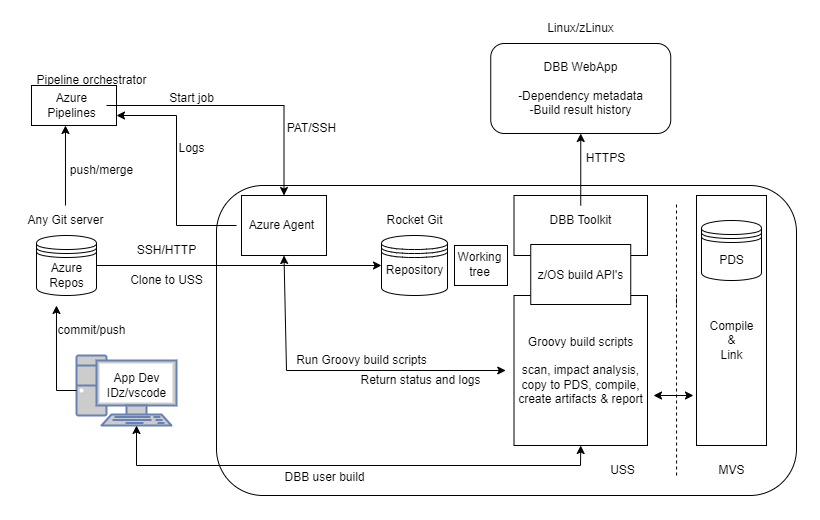
\includegraphics[scale=0.5]{DBB_architecture}
    \caption{DBB architectuur van dit onderzoek}
    \label{fig:dbb architectuur}
\end{figure}
\\ \\
\section{Azure DevOps}
\label{sec:azure devops}
\subsection{Wat is Azure DevOps?}
Volgens \textcite{Microsoft2024} ondersteunt Azure DevOps de samenwerking van ontwikkelaars, projectmanagers en medewerkers door een reeks processen aan te bieden die gebruikt worden om software te ontwikkelen. Het stelt organisaties in staat om sneller producten te maken en te verbeteren dan mogelijk is met traditionele softwareontwikkelingsmethoden.
\\ \\
Azure DevOps biedt geïntegreerde functies waartoe je toegang hebt via je webbrowser of IDE-client. Je kunt alle services gebruiken die bij Azure DevOps worden geleverd of alleen die services kiezen die je nodig hebt om je bestaande workflows aan te vullen.
\\ \\
\subsubsection{Azure producten}
Azure DevOps is een verzameling van vijf individuele services die samen de DevOps ontwikkel filosofie omarmt. Omdat de services onder de Azure DevOps suite zitten is communicatie tussen de services heel snel en heel eenvoudig op te zetten zonder gecompliceerde methodes om de communicatie tot stand te brengen.
\\ \\
Onder de \textcite{Microsoft2024} Azure DevOps suite zitten de volgende services:
\begin{itemize}
    \item Azure Boards: levert een suite van Agile tools om werk, code defecten en problemen te plannen en op te volgen, gebruikmakend van Kanban en Scrum methodes.
    \item Azure Repos: voorziet Git repositories of Team Foundation Version Control (TFVC) voor de source control van code.
    \item Azure Pipelines: voorziet build en release services om Continuous Integration (CI) en Continuous Delivery (CD) van applicaties te ondersteunen.
    \item Azure Test Plans: set van tools om applicaties te testen, inclusief manueel/exploratieve testing en continuous testing.
    \item Azure Artifacts: teams kunnen hier gebruik van maken om het delen van packages zoals Maven, npm, NuGet en andere packages van private- of publieke sources te integreren in pipelines.
\end{itemize}
Voor dit onderzoek zal er enkel gebruik gemaakt worden van de Azure Repos en Azure Pipelines services.
\\ \\
\subsection{Azure Repos als Source Code Control}
In Azure Repos zijn er twee manieren om aan Source Code Control te doen, via Team Foundation Version Control (TFVC) of via Git (gedistribueerd). TFVC is een gecentraliseerd client-server systeem. In zowel Git als TFVC kan er gebruik gemaakt worden van folders, branches en repositories om bestanden te organiseren. Voor dit onderzoek zal er gebruik gemaakt worden van een gedistribueerd Source Code Control (Git) \autocite{Microsoft2022}.
\\ \\
Via Azure Repos kan je alle repositories waartoe je toegang hebt beheren en eventueel aanpassen. Zo kunnen er branches, tags (versies), commits, pushes, merges en pull requests aangemaakt worden. Er kunnen ook handmatig, via Azure Repos, bestanden of folders geüpload worden \autocite{Microsoft2022}.
\\ \\
Azure Repos heeft ook de functionaliteit om automatisch of handmatig applicaties een nieuwe versie te bezorgen na een push. Zo kan er ook aan versiebeheer gedaan worden binnen Azure Repos, er kan ten allen tijden teruggegaan worden naar een vorige versie of commit. Op die manier hoef je niet expliciet meerdere versies bij te houden van eenzelfde applicatie en kan er bij problemen altijd teruggegaan worden naar een vorige werkende versie \autocite{Microsoft2022}.
\\ \\
Een ontwikkelaar die werkt met Azure Repos heeft een eigen kopie van de source repository op zijn computer. De source repository komt inclusief met alle branches en vorige versies van de repository. De ontwikkelaar werkt rechtstreeks op zijn eigen lokale repository en de aanpassingen worden gedeeld naar de centrale repository door een push naar de main source repository. Op die manier kan de ontwikkelaar zelf aan versiebeheer doen door de vorige versies te vergelijken met elkaar zonder netwerk connectie \autocite{Microsoft2022}.
\\ \\
Wanneer de ontwikkelaar een nieuw onderdeel wil toevoegen aan de applicatie kan die ook zijn eigen lokale branch maken om daarop verder te werken zonder andere ontwikkelaars te dwarsbomen. Doordat de branches lichtgewichten zijn op vlak van opslag kan er snel en makkelijk gewisseld worden tussen branches. Indien de ontwikkelaar klaar is met zijn onderdeel kan die door middel van een push/merge de main branch updaten met zijn nieuwe code, zo kan zijn lokale branch opgeruimd worden na de push/merge \autocite{Microsoft2022}.
\\ \\
\subsection{Azure Pipelines als pipeline orchestrator}
Azure Pipelines zorgt ervoor dat het mogelijk is om meerdere taken opeenvolgend te automatiseren om op die manier het builden en deployen van applicaties makkelijker en gestroomlijnder te maken. Met Azure Pipelines kan je taken zoals bestanden aanmaken en scripts of commando's uitvoeren, automatiseren in één of meerdere pipelines. Zo kan er met Azure Pipelines een systeem opgezet worden dat na afloop van een pipeline er opnieuw een pipeline zal gestart worden. Dit kan automatisch of manueel ingesteld worden. Het is ook mogelijk om Azure Pipelines je Git repository in Azure Repos te laten observeren en wanneer die een verandering detecteert in de source code, wordt er automatisch een pipeline gestart. Dit maakt het mogelijk om aan Continuous Integration (CI) te doen en doordat de mogelijkheid bestaat om meerdere pipelines/taken na elkaar uit te voeren kan er ook gedaan worden aan Continuous Delivery (CD). \autocite{Microsoft2023}
\\ \\
Een ontwikkelaar die werkt met Azure Pipelines hoeft, indien de optie CI aanstaat voor de repository en pipeline, enkel maar een push uit te voeren naar de repository en dan activeert die push de pipeline die daaraan gekoppeld is. De taken van de pipeline worden dan zelfstandig uitgevoerd zonder dat de ontwikkelaar zelf iets moet selecteren of uitvoeren. Er kan ook manueel een pipeline gestart worden, eenmaal gestart werkt die op dezelfde manier als de pipeline die geactiveerd werd door een push naar de gelinkte repository. \autocite{Microsoft2023}
\\ \\
Standaard is er ondersteuning om controle mechanismen in te schakelen binnenin de pipeline. Zo kan er voordat de pipeline effectief verandering brengt in bijvoorbeeld een productie applicatie eerst een review gevraagd worden aan een of meer leidinggevenden. Pipelines kunnen ook afgeschermd worden van bepaalde personen of groepen om zo confidentialiteit te waarborgen. \autocite{Microsoft2023}
\\ \\
Azure Pipelines hebben ook de mogelijkheid om automatische testing in gang te zetten bij het uitvoeren van de pipeline. Zo kan er naargelang het resultaat van de testen alsnog de wijziging van een applicatie afgebroken worden. Indien de pipeline succesvol beëindigd wordt kan er ook een optie aangevinkt worden om automatische versie controle aan te zetten. Zo kan er bij een applicatie van versie 1.0.1 na een succesvolle uitvoering van de pipeline de versie 1.0.2 meegegeven worden. \autocite{Microsoft2023}
\\ \\ \\ \\ \\ \\
\section{Git workflows}
\subsection{Software Development Lifecycle}
Een van de belangrijkste aspecten van mainframe software ontwikkeling is dat het betrouwbaar, beschikbaar en bruikbaar is. Deze workflow zit nagenoeg standaard ingebakken in mainframe softwareontwikkeling, maar hoe kan die workflow gerecreëerd of zelfs verbeterd worden door middel van gebruik te maken van Git om de softwareontwikkeling workflow op te stellen. Volgens Nelson \textcite{Lopez2023} is een van de beste strategieën om dezelfde eigenschappen van een mainframe workflow te bekomen om de Software Development Lifecycle te recreëren met behulp van Git, een Git ondersteunende IDE, CI pipeline, deployment policies en een CD pipeline.
\\ \\
Op de manier zoals voorgesteld door \textcite{Lopez2023} zou de source code storage niet meer in PDS's opgeslagen worden maar in een Git gedistribueerd bestandssysteem, versiebeheer zal niet meer verlopen via een SCM package ID maar via Git commit ID of Git tags. Indien er wijzigingen moeten aangebracht worden in de source code wordt er geen ISPF maar een IDE zoals vscode of IDz, de compile/link van een programma zal dan weer verzorgd worden door een CI pipeline en niet door een JCL. Toestemmingen en het aanvaarden van wijzigingen aan applicaties zal je dan weer kunnen doen door middel van Git merge en deployment policies in plaats van de SCM. Als laatste zal het uiteindelijk deployen van een programma niet via JCL gebeuren maar via een CD pipeline.
\begin{figure}[h]
    \centering
    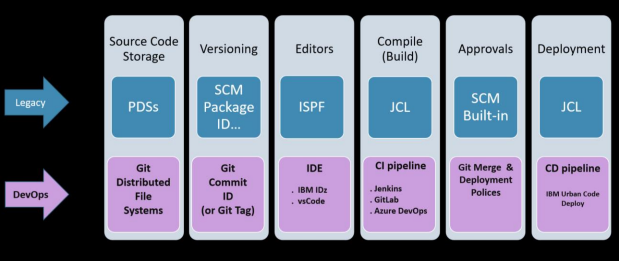
\includegraphics[scale=0.75]{Software_development_lifecycle}
    \caption{Software Development Lifecycle: Legacy vs DevOps \autocite{Lopez2023}}
    \label{fig:software development lifecycle}
\end{figure}
\\ \\ \\ \\
\subsection{Git branching strategie}
Elk bedrijf regelt zijn software ontwikkeling op een manier zodat er een duidelijk onderscheid en doel is voor elke omgeving. Zo is er een productieomgeving, de lopende versie van een applicatie zit daar te draaien. Er is ook een development omgeving waarin nieuwe features of verbeteringen voor die applicatie worden ontwikkeld. Tot slot is er ook nog de QA omgeving (Quality Assesment) deze omgeving wordt gebruikt om applicaties te testen op functioneel vlak vaak tegenover de productie database.
\\ \\
Om een goede branching strategie te bekomen is het belangrijk volgens \textcite{Lopez2023} dat tenminste die drie omgevingen worden geïmplementeerd als een branch in de branching strategie. Dit komt neer op een main (productie) branch, een develop (development/ontwikkeling) branch en een release (QA) branch.
\\ \\
Om nog beter te werk te gaan moeten er nog een aantal zaken toegevoegd worden aan de branching strategie zo heeft Nelson Lopez het onder andere over een feature en hotfix/nood branch. Die laatste is voor noodgevallen waarin er heel snel iets veranderd moet worden aan de applicatie die in productie draait. De feature branch zou dan weer een lokale branch worden waarin de ontwikkelaar werkt aan zijn opdracht voor die applicatie. De workflow die wordt beschreven door Nelson Lopez is visueel te vinden in figuur \ref{fig:git branching strategie}.
\begin{figure}[h]
    \centering
    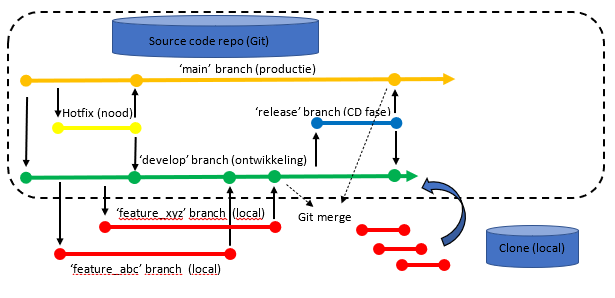
\includegraphics[scale=0.75]{Git_branching_strategy}
    \caption{Git branching strategie beschreven door Nelson Lopez}
    \label{fig:git branching strategie}
\end{figure}
\\ \\
De weg die een applicatie aflegt binnen de strategie die afgebeeld wordt op \ref{fig:git branching strategie} begint bij het binnenhalen van de applicatie versie die in de ontwikkelomgeving draait. Die is te vinden op de develop branch, vandaar wordt er een clone gemaakt naar een lokaal werkstation en wordt allereerst een nieuwe feature branch aangemaakt. De naamgeving van die branch kan als volgt zijn: feature-array-toevoegen, dit is afhankelijk van de policy binnen de werkomgeving omtrent naamgeving van branches.
\\ \\
Eenmaal de feature branch aangemaakt is kan de ontwikkelaar aan het werk gaan om de feature te coderen. In de tussentijd kan er een andere ontwikkelaar aan hetzelfde programma werken op nog een andere feature branch. Die ontwikkelaar moet bijvoorbeeld foutmeldingen aanpassen dus zijn feature branch krijgt de naam feature-update-foutmeldingen. Als een ontwikkelaar klaar is met zijn feature dan kan die een merge uitvoeren naar de develop branch om de versie die daar draait te updaten met zijn aangepaste versie. Doordat Git een merge functie heeft gaat Git enkel hetgeen aanpassen dat de ontwikkelaar zelf heeft gewijzigd. Zo kan er tussendoor iemand anders al een merge uitgevoerd hebben naar diezelfde branch zonder dat er conflicten zijn.
\\ \\
Nadat een applicatie in de ontwikkelomgeving een of meerdere updates heeft gekregen kan er gekozen worden om die versie over te zetten naar de productie omgeving. Voordat effectief plaatsvindt zal er eerst een release branch aangemaakt worden om de functionele testen uit te voeren en indien nodig source code aan te passen. Pas als de testen vlot verlopen dan wordt er zowel met de main branch (productie) als met de develop branch een merge uitgevoerd. Zo zijn beide versies up to date met de versie die doorheen de functionele test fase is geraakt (QA).
\\ \\
In geval dat er een situatie is waarin de productie versie niet meer draait dan wordt er een hotfix branch gemaakt vanaf de versie die draait op productie. Source code wordt aangepast en testing wordt opnieuw uitgevoerd zoals bij de release branch. Indien die testen succesvol zijn dan wordt de aangepaste versie zowel met de main branch als met de develop branch gemerged. Hierdoor wordt de fout die in de productie versie zat zowel in de ontwikkelomgeving als in de productieomgeving opgelost.
\\ \\
%%=============================================================================
%% Methodologie
%%=============================================================================

\chapter{\IfLanguageName{dutch}{Methodologie}{Methodology}}%
\label{ch:methodologie}
\section{Fase 1: Literatuurstudie}
\label{sec:Fase 1: Literatuurstudie}
In de eerste fase van dit onderzoek wordt er een uitgebreide literatuurstudie gemaakt. Deze literatuurstudie zal gebruikt worden als voornaamste gegevensbron voor het verdere verloop van het onderzoek. De literatuurstudie heeft drie grote onderwerpen namelijk de mainframe, RESTfull APIs en z/OS Connect. In het hoofdstuk omtrent de mainframe zal er gekeken worden wat een mainframe is, waarvoor het gebruikt wordt en wat de geschiedenis ervan is.
\\ \\
In het stuk over RESTfull APIs zal er beschreven worden wat een API is, hoe een API RESTfull kan worden en waarvoor RESTfull APIs gebruikt kunnen worden. Verder zal er ook te vinden zijn wat een API consumer is en wat een API provider is, er zal ook te vinden zijn wat de verschillende componenten zijn van een API.
\\ \\
In het laatste deel van de literatuurstudie zal het gaan over z/OS Connect. Hierin worden een aantal onderwerpen aangeraakt, wat is z/OS Connect, wat zijn de components ervan en hoe z/OS Connect werkt. Ook zal er beschreven zijn waarvoor z/OS Connect wordt gebruikt, wat de architectuur ervan is en op het einde van het deel over z/OS Connect is er een beschrijving van de installatie en configuratie ervan.
\\ \\
Na de eerste fase, die geschat is op twee weken, is er een diepgaande en volledige literatuurstudie die de rode draad zal zijn wat betreft informatie in het onderzoek.
\\ \\
\section{Fase 2: Voorbereiding installatie}
\label{sec:Fase 2: Voorbereiding installatie}
Het doel van de volgende fase is om gedurende een week het systeem klaar te krijgen voor de installatie, dit wordt bekomen door het controleren van alle vereisten om het installatieproces te kunnen starten. Aan de hand van die vereisten wordt er gekeken of het systeem nog een aantal aanpassingen nodig heeft. Pas daarna kan er overgegaan worden op de effectieve installatie van z/OS Connect. Dit proces zal enkel theoretisch worden besproken aangezien Arcelor Mittal zijn mainframe niet zelf onderhoud en dus niks zelfstandig mag installeren op hun mainframe.
\\ \\
\section{Fase 3: Installatie}
\label{sec:Fase 3: Installatie}
De derde fase stelt de installatie van z/OS Connect voor, deze fase zal sterk profiteren van het voorbereidende werk dat in fase twee is gebeurd. Het installatieproces wordt geschat op anderhalve week. Na de installatie is het systeem klaar om volledig geconfigureerd te worden. Hier wordt opnieuw enkel theoretisch over gesproken in de thesis.
\\ \\
\section{Fase 4: Configuratie}
\label{sec:Fase 4: Configuratie}
Na de installatie komt de configuratie, er worden allerhande instellingen geconfigureerd van z/OS Connect zo gaat die naadloos kunnen werken met de huidige mainframe architectuur van Arcelor Mittal Gent. De configuratie wordt uitvoerig getest en dat is dan ook de reden dat deze fase twee en een halve week in beslag neemt. Pas als alle functies van z/OS Connect operationeel zijn kan er overgegaan worden om met z/OS Connect te experimenteren.
\\ \\
\section{Fase 5: Proof of Technologies}
\label{sec:Fase 5: Proof of Technologies}
Er wordt anderhalve week voorzien om even te experimenteren met z/OS Connect en de mogelijkheden ervan eens op de proef te nemen. Deze testen zullen vooral gaan over de ingebouwde APIs en calls die het al bevat. Al zal er ook gekeken worden naar de mogelijkheden die er zijn om eigen calls en APIs te schrijven. Na deze fase kan er overgegaan worden naar de uitzetting van de Proof Of Concept.
\\ \\
\section{Fase 6: Proof of Concept}
\label{sec:Proof of Concept}
De uitzetting en realisatie van de POC is een heel belangrijke fase omwille van het feit dat hier de resultaten worden bekomen om een conclusie te trekken op het einde van dit onderzoek. De opdracht bestaat erin om een applicatie, dat niet noodzakelijk een COBOL of PL/I applicatie is, te laten communiceren met de mainframe resources. Zo zal er gekeken worden of een applicatie een bestand kan lezen of aanpassen alsook datzelfde bestand te verwijderen. De gebruiker moet natuurlijk wel de juiste rechten hebben om de gevraagde zaken te kunnen doen. Als die niet de juiste rechten heeft dan moet de gevraagde actie geweigerd worden. De gebruiker moet ook een nieuw bestand kunnen aanmaken met behulp van z/OS Connect, opnieuw rekeninghoudend met de rechten van die gebruiker. Dit alles wordt gestuurd door een .NET applicatie, de communicatie is dus over twee verschillende platformen heen. Deze communicatie kan langs beide kanten gaan, zo kan een mainframe applicatie een .NET applicatie oproepen en andersom. Na deze twee en een half week durende fase is alle informatie om een conclusie te trekken aanwezig.
\\ \\
\section{Fase 7: Resultaten analyse}
\label{sec:Fase 7: Resultaten analyse}
De volgende fase van dit onderzoek is om de resultaten die doorheen dit onderzoek zijn bekomen te analyseren. Deze analyse wordt niet gedaan door de developers maar door verschillende business analisten. Al zal er wel gevraagd worden aan de developers en eindegebruikers wat zij vinden van de resultaten van het onderzoek. Zo kan het zijn dat een gebruiker blij is met de resultaten omdat die zijn werkgemak heeft verbeterd door het werken met z/OS Connect. Deze analyse zal 1 week in beslag nemen.
\\ \\
\section{Fase 8: Conclusie}
\label{sec:Fase 8: Conclusie}
Na de resultaten analyse volgt de fase waarin er conclusies worden getrokken, dit zal afhankelijk van de beslissing van de analisten ofwel de volledige uitrolling van z/OS Connect zijn of dan toch het niet gebruiken van z/OS Connect. Voor deze fase wordt er 1 week gerekend.
\\ \\
\section{Fase 9: Scriptie afwerken}
\label{sec:Fase 9: Scriptie afwerken}
De laatste fase is om de scriptie af te werken, zo zal er in die week gekeken worden om alle puntjes op de i te zetten en alles nog eens goed na te kijken alvorens in te dienen.
\\ \\
\section{Gantt chart}
Hieronder een Gantt chart met alle fasen nog eens weergegeven op een visuele manier.

\begin{center}
    \hspace*{-1.5cm}%
    \begin{ganttchart}[
        vgrid,
        bar label node/.append style={align=right}
        ]{1}{28}
        %labels
        \gantttitle{Week}{28} \\
        \gantttitle{1}{2}
        \gantttitle{2}{2}
        \gantttitle{3}{2}
        \gantttitle{4}{2}
        \gantttitle{5}{2}
        \gantttitle{6}{2}
        \gantttitle{7}{2}
        \gantttitle{8}{2}
        \gantttitle{9}{2}
        \gantttitle{10}{2}
        \gantttitle{11}{2}
        \gantttitle{12}{2}
        \gantttitle{13}{2}
        \gantttitle{14}{2}\\
        %tasks
        \ganttbar{Literatuurstudie maken}{1}{3} \\
        \ganttbar{Vereisten nakomen}{4}{5} \\
        \ganttbar{Installatie z/OS Connect}{6}{8} \\
        \ganttbar{Configuratie z/OS Connect}{9}{13} \\
        \ganttbar{Experimentatie z/OS Connect}{14}{16} \\
        \ganttbar{Uitzetten en realiseren POC}{17}{22} \\
        \ganttbar{Resultaten analyse}{23}{24} \\
        \ganttbar{Conclusie}{25}{26} \\
        \ganttbar{Scriptie afwerken}{27}{28} \\

        %relations
        \ganttlink{elem0}{elem1}
        \ganttlink{elem1}{elem2}
        \ganttlink{elem2}{elem3}
        \ganttlink{elem3}{elem4}
        \ganttlink{elem4}{elem5}
        \ganttlink{elem5}{elem6}
        \ganttlink{elem6}{elem7}
        \ganttlink{elem7}{elem8}
    \end{ganttchart}
    %    \caption{Gantt Chart}
    \hspace*{-1.5cm}%
\end{center}



% Voeg hier je eigen hoofdstukken toe die de ``corpus'' van je bachelorproef
% vormen. De structuur en titels hangen af van je eigen onderzoek. Je kan bv.
% elke fase in je onderzoek in een apart hoofdstuk bespreken.

%%=============================================================================
%% PROOF-OF-CONCEPT
%%=============================================================================

\chapter{\IfLanguageName{dutch}{Werking huidig systeem}{Operation of the current system}}%
\label{ch:current system)}

\section{Inleiding}
\label{sec:inleiding_currsys}
Dit hoofdstuk zal de werking van het huidige systeem om coolgen applicaties te ontwikkelen van ArcelorMittal Gent toelichten en visualiseren. De stappen die in het huidige systeem aanwezig zijn zullen ook terug te vinden zijn in het nieuwe systeem met behulp van een pipeline en IBM DBB. Het is uiterst noodzakelijk om kennis te hebben van het huidige systeem alvorens een nieuw systeem kan gemaakt/geïmplementeerd worden. Dit komt doordat het systeem dat momenteel gebruikt uitermate veel is gepersonaliseerd door ArcelorMittal Gent om aan hun eisen en gebruiken te voldoen. 

\section{Compileren}
\label{sec:compileren}
De huidige geïnstalleerde versie van de Cobol compiler binnen ArcelorMittal Gent is versie 6.20, deze versie van Cobol is geïntroduceerd in 2017 op 8 september en heeft geen support meer vanaf 30 september 2024.
\\ \\
De JCL die uitgevoerd wordt wanneer men een compilatie van een programma wil uitvoeren wordt opgeroepen via een product van Rocket software namelijk MSP (Manager Products). Dit product zorgt ervoor dat een ontwikkelaar kan meegeven welk programma hij/zij wil compileren en in welke omgeving die dat wil doen, dit kan bijvoorbeeld productie of ontwikkeling zijn. Dat product zorgt er dan voor dat de JCL voor de compile uit te voeren wordt gestart met de juiste parameters en de juiste libraries die moeten meegegeven worden tijdens de compilatie zoals de SYSLIB en SYSIN DD's.
\\ \\
Heel belangrijk binnen het huidig systeem is het gebruik van meta-data, hierdoor weet in dit geval MSP welke parameters die moet aanvoeren aan de compiler, welke libraries die moet alloceren en of er extra zaken moeten gestart worden zoals een Db2 package bind of Db2 plan bind. Deze meta-data is dan ook een van de eerste zaken dat gecontroleerd wordt als men een compilatie wil starten. Indien er geen meta-data te vinden is dan zal de compile geannuleerd worden. 
\\ \\
Deze meta-data bevat onder andere informatie over de afdeling waar het gemaakt is, de programmeur van de applicatie, wat voor soort applicatie het is. Zo heb je 3 verschillende soorten programma's binnen ArcelorMittal Gent, je hebt de main programma's, die kunnen ofwel volledig onafhankelijk draaien of ze roepen sub programma's op. Deze main applicaties kunnen zelf niet opgeroepen worden door andere applicaties. Als laatste zijn er ook nog 2 soorten sub programma's, de fsub en de sub. In theorie is er niet veel verschil buiten de manier waarop ze opgeroepen kunnen worden. Zo wordt een sub statisch gebindt aan een programma dat hem oproept en een fsub wordt dynamisch opgeroepen tijdens de run time. Naast die 3 soorten van applicaties is er ook nog het feit of er gebruik gemaakt wordt van subsystemen zoals IMS, Db2 of MQ. Indien hiervan gebruik gemaakt wordt dan kan de ontwikkelaar ook deze zaken aanduiden binnen het meta-data scherm van zijn/haar applicatie. 
\\ \\
Eenmaal alle meta-data aanwezig is zal MSP met behulp van skeletons de juiste JCL opmaken om die applicatie te compileren met de juiste libraries en parameters. De compile parameters zijn heel gelijkaardig voor alle soorten programma's maar kunnen toch nog ergens licht afwijken. Zoals wanneer er gebruik gemaakt wordt van een subsysteem zoals IMS of Db2.
\\ \\

\section{Bind}
\label{sec:bind}
Er wordt gebruik gemaakt van de IEWL Binder voor z/OS 2.5 om de applicaties van ArcelorMittal te binden. Het belangrijkste verschil tussen een programma dat gebind is met IEWL en een dat gelinkedit is, is het feit dat bij de linkedit een groot uitvoerbaar bestand gemaakt wordt van de verschillende objectbestanden van het hoofdprogramma, de subprogramma's en de subroutines die opgeroepen worden. Hierdoor is het programma dat gelinkedit wordt statisch aangemaakt, dit wil zeggen dat indien er een sub programma verandert er dus een nieuwe linkedit moet gebeuren van alle progamma's die dat sub programma gebruiken. Met een binder kan je dynamisch een programma aan een ander programma koppelen/binden, op die manier is het zo dat een sub programma opgeroepen wordt op run time en niet tijdens de compile. Hierdoor hoeft er geen herlink meer te gebeuren van de applicaties die dat programma gebruiken. 
\\ \\
Er zijn net zoals bij de compilatie ook parameters die meegegeven worden aan de binder om op de juiste manier de programma's te kunnen binden. In tegenstelling als bij de compilatie moet er niet voor elk soort programma (main, Db2, IMS, sub, ...) een aparte parameter lijst gemaakt worden. De parameters zijn hetzelfde voor main- en fsub programma's aangezien die worden opgeslagen als DLL, voor de sub programma's is er een andere parameter lijst die ervoor zorgt dat de sub geen DLL wordt maar statisch blijft. Hierdoor zullen main- en fsub programma's wel dynamisch opgeroepen kunnen worden tijdens run time en zal er voor sub programma's opnieuw met herlink en hercompile moeten gewerkt worden. 
\\ \\ 
De binder wordt net zoals de compiler opgeroepen door het product MSP, het gaat op dezelfde manier te werk als bij de compile en maakt gebruik van een applicatie zijn meta-data om zo de juiste libraries en parameters mee te geven.

\chapter{Proof Of Concept}
\label{ch:poc}

\section{Inleiding}
\label{sec:inleiding_poc}
Het hoofdstuk van de Proof Of Concept zal gaan over welke stappen en producten er allemaal nodig waren om de proefopstelling succesvol te laten werken. Deze stappen zullen overeenkomen met die van het huidige systeem besproken in het vorige hoofdstuk.
\\ \\

\section{Installatie \& configuratie IBM DBB}
\label{sec:installdbb}
De eerste stap in het opzetten van de proefopstelling is om de IBM DBB installatie af te ronden en de configuratie te starten. De installatie op de mainframe van ArcelorMittal werd gedaan door een bedrijf genaamd NRB, zij zijn verantwoordelijk voor installatie van software op de mainframe van ArcelorMittal Gent. 
\\ \\
Aangezien IBM DBB al geïnstalleerd is voor deze Proof Of Concept kan er direct begonnen worden aan de configuratie van de bestanden die gebruikt worden door het product DBB. Deze bestanden zijn onder andere properties bestanden die ervoor zorgen dat bepaalde zaken zoals de binder en compiler worden gedeclareerd. Deze zijn niet standaard meegeleverd en moeten afgehaald worden vanaf een git repository namelijk de dbb-zappbuild git repository van IBM. 
\\ \\
\subsection{Installatie dbb-zappbuild}
Die repository kan rechtstreeks gecloned worden of via file transfer kunnen die ook op de juiste plaats in de USS belanden. De aanbevolen plaats om die repository te stockeren is in de hoofdfolder van DBB, dat ziet eruit zoals /dbb/dbb-zappbuild.
\\ \\
\subsection{Configuratie dbb-zappbuild}
Nu dat de dbb-zappbuild repository aanwezig is op de USS kan er begonnen worden aan de configuratie van DBB. Deze configuratie op de USS bestaat hoofdzakelijk uit properties en .groovy bestanden. De properties bestanden zijn te vinden in de folder build-conf en zijn ook de eerste die moeten veranderd of ingevuld worden. Verder zijn er de .groovy bestanden die voor de verwerking van die properties zorgen, dit is in een hoofdprogramma (build.groovy), language specifieke programma's zoals Cobol.groovy en utility programma's zoals BuildUtilities.groovy.
\\ \\
Deze bestanden hebben elk hun eigen taken en nut in de werking van het systeem, zo zijn de properties bestanden noodzakelijk om datasets en PDS'en mee te geven om zo de juiste binder, compiler, load libraries en dergelijke te hebben. De taak van een language specifiek groovy programma zoals Cobol.groovy is om de compilatie en bind van een programma dat in die taal geschreven is uit te voeren. Dit kan heel erg verschillen tussen talen door, zo is de compilatie van een PL/I programma een stuk anders dan de compilatie van een Cobol programma. De zaken die nodig zijn om die compilatie en bind goed uit te voeren kunnen gevonden worden in zo'n language specifiek groovy programma. Deze language specifieke programma's gebruiken heel vaak utility programma's om zaken die hetzelfde zijn in elke taal te bundelen zo is er een BindUtilities.groovy dat een DB2 package bind en/of plan bind kan doen. Dit is onafhankelijk van welke taal je gebruikt en kan dus in zo'n utility programma. Als laatste om de cyclus te vervolledigen is er de build.groovy, dit is het hoofdprogramma dat alle andere programma's op de juiste moment oproept.
\\ \\
\begin{figure}[h]
\begin{tabularx}{1\textwidth} { 
        | >{\centering\arraybackslash}X 
        | >{\centering\arraybackslash}X 
        | >{\centering\arraybackslash}X 
        | >{\centering\arraybackslash}X  | }
    \hline
    Properties bestanden & 
    Language groovy bestanden & 
    Utility groovy bestanden & 
    build.groovy \\
    \hline
    Dataset en PDS declaratie & 
    Oproepen van utilities en language specifieke werking bepalen & 
    Werking van language onafhankelijke procedures bepalen & 
    Oproepen van de juiste groovy sub programma's \\ 
    \hline
\end{tabularx}
\caption{Soorten bestanden en hun taak}
\label{tab:soorten bestanden}
\end{figure}

\subsubsection{Properties bestanden}
Er zijn in totaal 16 properties bestanden waarin aanpassingen moeten aangebracht worden deze zijn onderverdeeld in de verschillende talen en gebruiken. Zo zijn er properties bestanden voor Cobol, PL/I, PSB, ACB en nog een aantal anderen. Er is ook een datasets.properties bestand waarin veel algemene PDS'en en datasets worden gedeclareerd. Zo kan je bijvoorbeeld de z/OS macro library, Cobol compiler, PL/I compiler en DB2 load library vinden en declareren in de datasets.properties. 
\\ \\
In de build.properties zit er vooral algemene instellingen en dus geen datasets, zo kan je aanduiden welke properties bestanden ingeladen kunnen worden als het systeem geactiveerd word. Deze zit net zoals de datasets.properties en de overige taal- en gebruiksspecifieke properties bestanden in de build-conf folder die te vinden is binnen de dbb-zappbuild map. 
\\ \\
De taal specifieke properties worden aangepast in onder andere Cobol.properties en de PLI.properties bestanden. Hierin worden onder andere instellingen zoals load libraries, vereiste properties en compiler opties meegegeven die algemeen gelden voor alle programma's van die taal. De volledige properties bestanden zijn te vinden in appendix \ref{ch:appropsbuild}.
\\ \\
\subsubsection{Language groovy bestanden}
De language groovy bestanden zorgen ervoor dat de programma's van die taal succesvol gecompileerd en gebind kunnen worden. Naast de compile en bind wordt er ook gezorgd dat de load module van de applicatie op de juiste plaats beland, dat er een DB2 package bind en/of plan bind uitgevoerd wordt indien nodig. Zo wordt ervoor gezorgd dat het programma niet alleen goed wordt gecompileerd en gebind maar ook uitvoerbaar is op het mainframe van ArcelorMittal Gent. Binnen dit onderzoek is het enigste language groovy programma de Cobol.groovy, het volledige aangepaste script is te vinden in appendix \ref{ch:aplangroovy}.
\\ \\
\subsubsection{Utility groovy bestanden}
De utility groovy programma's worden door zowel de language groovy bestanden als de build.groovy opgeroepen om language onafhankelijke procedures op te roepen. Zo is er een groovy utility programma dat ervoor zorgt dat onder andere de build lijst wordt aangemaakt, meta data wordt ingevuld, logicalfiles worden aangemaakt en ervoor zorgt dat datasets kunnen aangemaakt worden. Dit is maar een kleine opsomming van de mogelijkheden van de BuildUtility.groovy, hiernaast zijn er nog 7 andere groovy utility programma's. De enigste programma's die aangepast zijn in het kader van het onderzoek zijn BuildUtilities.groovy en BindUtilities.groovy, deze zijn te vinden in appendix \ref{ch:aputilgroovy}. 
\\ \\
\subsubsection{build.groovy}
Dit groovy programma roept andere programma's op zoals de utility programma's en de language specifieke programma's. Er wordt een build lijst gemaakt op basis van de rangschikking die meegegeven wordt binnen de properties van de build. Er worden dus groovy bestanden aangeroepen en de properties worden ingeladen zodat die gebruikt kunnen worden door de build.groovy en de andere groovy programma's. 
\\ \\
Hieronder een opsomming van alle bestanden en programma's die ervoor zorgen dat DBB de programma's en bestanden kan compileren, binden en opslaan in een z/OS omgeving.
\begin{multicols}{2}
    \begin{itemize}
        \item \textbf{Properties bestanden}
        \begin{itemize}
            \item ACBgen.properties
            \item Assembler.properties
            \item build.properties
            \item Cobol.properties
            \item datasets.properties
            \item DBDgen.properties
            \item defaultzAppBuildConf.properties
            \item dependencyReport.properties
            \item LinkEdit.properties
            \item MFS.properties
            \item PLI.properties
            \item PSBgen.properties
            \item Transfer.properties
            \item ZunitConfig.properties
        \end{itemize}
        
        \item \textbf{Language groovy bestanden}
        \begin{itemize}
            \item Assembler.groovy
            \item Cobol.groovy
            \item DBDgen.groovy
            \item LinkEdit.groovy
            \item MFS.groovy
            \item PLI.groovy
            \item PSBgen.groovy
            \item Transfer.groovy
            \item ZunitConfig.groovy
        \end{itemize}
        
        \item \textbf{Utility groovy bestanden}
        \begin{itemize}
            \item BindUtilities.groovy
            \item BuildUtilities.groovy
            \item BuildReportUtilities.groovy
            \item DependencyScannerUtilities.groovy
            \item FilePropUtilities.groovy
            \item GitUtilities.groovy
            \item ImpactUtilities.groovy
            \item ReportingUtilities.groovy
        \end{itemize}
        
        \item \textbf{build.groovy}
    \end{itemize}
\end{multicols}
\\ \\
\subsection{Configuratie DBB buiten USS}
Naast de configuratie van DBB in de zapp-build op USS is er ook een configuratie die in elke repository meegegeven moet worden bij het starten van DBB. Dat zijn properties bestanden die in de repository meegeleverd moeten worden om de compilatie en bind in goed uit te voeren. Deze properties bestanden hebben altijd een application.properties en een file.properties, hierin wordt er onder meer een build lijst rangschikking meegegeven om te beslissen in welke orde programma's zullen gecompileerd worden. Naast de application- en file.properties moet er ook per taal een properties bestand meegegeven worden met extra instellingen die toegevoegd worden aan de al beschikbare instellingen die in de properties op USS zijn gedeclareerd. Zo moet er bij de verwerking van een Cobol programma de file-, application- en Cobol.properties bestanden aanwezig zijn binnen de repository. 
\\ \\
Er zijn in totaal voor ArcelorMittal 10 properties bestanden die meegegeven kunnen worden binnen een repository. Deze worden hieronder opgesomd.
\begin{multicols}{2}
    \begin{itemize}
        \item application.properties
        \item Assembler.properties
        \item Cobol.properties
        \item file.properties
        \item languageConfigurationMapping
        \item LinkEdit.properties
        \item PLI.properties
        \item reports.properties
        \item Transfer.properties
        \item ZunitConfig.properties
    \end{itemize}
\end{multicols}
\\ \\
Naast de properties bestanden is er nog een .gitattributes bestand dat heel belangrijk is in verband met het omzetten van de encodering van z/OS naar git en omgekeerd. Op de mainframe van ArcelorMittal Gent wordt er gebruik gemaakt van de EBCIDIC IBM 1148 encodering en die is niet standaard ondersteund door git. Daardoor moet er in een .gitattributes bestand aangegeven worden dat de input in die EBCIDIC encodering staat en dus nog moet omgezet worden naar UTF-8. De properties bestanden en .gitattributes die gebruikt worden binnen de repository van dit onderzoek zijn volledig aangepast terug te vinden in appendix \ref{ch:appropappli}. 

\pagebreak

\section{Opzetten pipeline Azure DevOps}
Om de compilatie en bind van programma's te voltooien wordt er gebruik gemaakt van pipelines en pipeline software om dat proces te starten. In dit onderzoek zal er gebruik gemaakt worden van Azure Pipelines, een product uit de Azure DevOps suite. De reden dat er gebruik gemaakt wordt van Azure Pipelines en niet van een andere pipeline software zoals Jenkins is door het feit dat ArcelorMittal Gent al een licentie had voor Azure DevOps. Zo wordt de software stack van ArcelorMittal niet onnodig uitgebreid. 

\subsection{Azure DevOps workflow}
Voordat er gestart kan worden moet er bekeken worden welke workflow er gebruikt zal worden binnen de pipeline en Azure DevOps. De workflow die gebruikt wordt in dit onderzoek is heel standaard en zal gaan van een desktop met IDz of Visual Studio Code naar het eindstation z/OS. Dit gaat als volgt te werk, er wordt begonnen vanaf niks dus er is nog geen enkele repository die op de desktop staat. 
\\ \\
De eerste stap is dus om een repository te clonen naar een lokale map, dit kan rechtstreeks vanuit IDz of Visual Studio Code. Dan wordt die repository lokaal aangepast door bijvoorbeeld een nieuwe branch toe te voegen, nieuwe commits of nieuwe code. Als de repository klaar is om doorgestuurd te worden naar z/OS dan wordt er via een ``git push'' een signaal verstuurd naar de centrale repository en die zal dan op zijn beurt een of meerdere pipeline jobs lanceren die uitgevoerd worden door een agent die ofwel op Linux of Windows draait. Die pipeline job zal de repository gaan clonen op z/OS, daarna wordt die repository met behulp van IBM DBB gebuild en de bekomen load modules en source files worden daarna op z/OS opgeslagen. De visuele weergave van deze workflow is te vinden op figuur \ref{fig:azure devops flow}.
\begin{figure}[h]
    \centering
    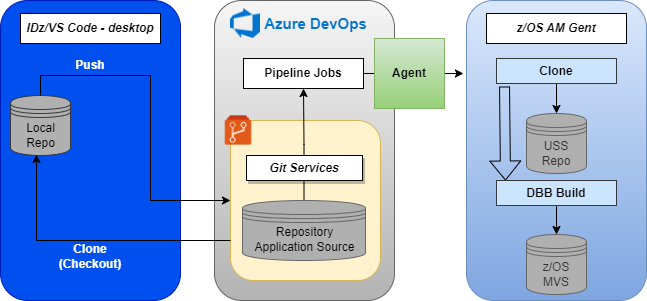
\includegraphics[scale=0.65]{AzureDevOps_Flow}
    \caption{Azure DevOps workflow}
    \label{fig:azure devops flow}
\end{figure}

\subsection{Opzetten van een organisatie, agent pool en agent in Azure DevOps}
Er wordt gewerkt binnen Azure DevOps met organisaties zo kan er op een makkelijke en overzichtelijke manier gescheiden gewerkt worden van andere takken en/of teams binnen een bedrijf. Voordat er kan begonnen worden aan het proces om een organisatie en agent op te zetten moet er toegang zijn tot Azure DevOps. Dit wil zeggen dat er een geregistreerd account ter beschikking moet zijn met de nodige privileges om een organisatie te mogen aanmaken. Indien dat ter beschikking is zouden er geen problemen mogen zijn met het opzetten van een organisatie en agent. 
\begin{enumerate}
    \item Inloggen op Azure DevOps.
    \item Aanmaken van een full acces \textbf{P}ersonal \textbf{A}cces \textbf{T}okens.
    \item Creëer een nieuwe organisatie.
    \item Toevoegen van een self hosted agent pool.
    \item Maken van een nieuwe agent op een Windows machine.
    \item Configureren van de Windows agent.
    \item Starten van de agent. 
\end{enumerate}
\autocite{Microsoft2024a}
\autocite{Microsoft2024b}
\autocite{Microsoft2024c}
\\ \\
Het nut van een agent pool en agents is om de pipelines uit te laten voeren. Elke agent kan 1 pipeline uitvoeren. Indien er twee pipelines zijn die uitgevoerd moeten worden, zal er een van de twee in een queue geplaatst worden totdat de agent terug beschikbaar is. Binnen een agent pool kunnen er meerdere agents geïnstalleerd zijn. Hierdoor is het mogelijk om meerdere pipelines tegelijk te laten uitvoeren binnen dezelfde agent pool. 
\\ \\
Het is mogelijk om restricties te plaatsen op agents of agent pools in verband met welke pipelines ze mogen/kunnen uitvoeren. Zo kan er een eigen agent pool zijn voor bijvoorbeeld een migratie pipeline en een voor de compilatie/bind van programma's. 

\subsection{Azure DevOps project en connectie met de mainframe}
Binnen een organisaties kunnen er meerdere projecten aangemaakt worden, zo kan er op een overzichtelijke manier gewerkt worden binnen Azure DevOps. Elk project heeft zijn eigen resources, zo kunnen er bijvoorbeeld meerdere Azure Repo's en Azure Pipelines aangemaakt worden per project. 
\\ \\
Naast de resources die al aan bod gekomen zijn is er ook de mogelijkheid om service connecties te leggen, in deze proof of concept werd dat gedaan naar de mainframe van ArcelorMittal Gent. Dit gebeurt binnen de project instellingen en dan service connections, op die manier kan er een SSH connectie gemaakt worden met een mainframe of bij uitbreiding een andere server/computer waarmee verbinding wenst gemaakt te worden. 
\\ \\
In het geval van dit onderzoek wordt er gebruik gemaakt van één project waarin geconnecteerd wordt naar de mainframe van ArcelorMittal Gent met behulp van de SSH service connectie. Voor de SSH verbinding moeten de juiste waarden ingevuld worden zoals host name en poort nummer. De authenticatie gebeurt via een RACF user en paswoord, zo is bij het onderzoek gebruik gemaakt van een persoonlijke user. Indien het paswoord van die user verandert zal ook de service connectie moeten aangepast worden naar het nieuwe paswoord.

\subsection{Azure Repo toewijzen aan een project}
Voordat er kan gewerkt worden op een remote repository moet er eerst een aangemaakt worden, dit gebeurt via het online portaal van Azure DevOps binnen het project waarin de repo aangemaakt dient te worden. 
\\ \\ 
Er kan gekozen worden om een nieuwe repo aan te maken of om te starten van een bestaande repository via een import, dit onderzoek zal starten vanaf een lege repository. 

\subsection{Azure Pipeline toewijzen aan een project}
De verbinding van de repository naar de mainframe wordt behandeld door een pipeline. Dit kan letterlijk gezien worden zoals de naam het aangeeft, het is een pijplijn waardoor allerhande informatie en bestanden wordt doorgegeven aan de repository, de user en de mainframe. 
\\ \\
Een pipeline wordt aangemaakt binnen een project en werkt door middel van bash scripts, de bash scripts die nodig zijn voor het werken met IBM DBB worden aangeboden door IBM in een document genaamd \enquote{Azure DevOps and IBM Dependency Based Build Integration}, hierin staan de voorgestelde scripts in vermeld. 
\\ \\
Het is aangeraden om te beginnen met een basisscript dat bijvoorbeeld de mappenstructuur toont of de aangemelde user alvorens te springen op de DBB scripts. De scripts van IBM werden aangepast naar de eisen van ArcelorMittal en wijken dus licht af ten opzichte van de originele scripts. Zowel de aangepaste als de originele scripts zijn te vinden in appendix \ref{ch:apbashpipe}.

\subsection{Testen werking pipeline}
Om er zeker van te zijn dat er over kan gegaan worden naar het gebruik van de IBM DBB bash scripts moet er zekerheid zijn dat de pipeline de goeie connectie maakt naar de mainframe en moet er ook gecloned kunnen worden binnen de USS. Met andere woorden Git moet daar goed geïnstalleerd zijn. Deze zaken kunnen makkelijk getest worden, het eerste wat getest is in dit onderzoek is of er wel degelijk een connectie was. Dat werd getest door een pipeline met het commando \enquote{whoami}, als dat de juiste user weergaf zoals opgegeven bij het aanmaken van de service connectie dan was er geen probleem. Indien die niet werd weergegeven dan is er iets fout gelopen bij de service connectie en moet die stap opnieuw gedaan/bekeken worden. 
\\ \\
Als er vastgesteld is dat er een connectie kan gemaakt worden met de mainframe is er in dit onderzoek gekeken naar Git op de USS. Daarvoor zijn er twee stappen namelijk zorgen dat Git geïnstalleerd is op de user die gebruikt wordt voor de service connectie en zorgen dat die user ook een Azure Repo kan clonen. 
\\ \\
Om te zien of Git geïnstalleerd is op de user zijn USS wordt het \enquote{git --version} commando gebruikt. Als dat een versie van git weergeeft wil dat zeggen dat Git geïnstalleerd is op die user zijn USS, indien er een boodsschap weergegeven wordt dat het commando niet gevonden werd dan is Git nog niet (goed) geïnstalleerd. 
\\ \\ 
Nadat vastgesteld is dat Git goed is geïnstalleerd kan de configuratie voor het clonen beginnen. De clone zal gebeuren aan de hand van een Personal Acces Token (PAT), met PAT kan er connectie gemaakt worden via HTTPS en niet via SSH. Eerste stap in dit proces is om een PAT aan te maken, dit kan via het Azure Repos dashboard door op de knop clone te klikken en dan git credentials aan te laten maken. Het paswoord dat gecreëerd wordt is uitermate belangrijk want deze wordt nergens bijgehouden door Azure DevOps om later terug op te vragen. Dat paswoord moet dan enkel nog omgezet worden naar een Base 64 encoding, dit kan via powershell op windows via de volgende commando's:
\begin{enumerate}
    \item \$MyPat='gekopieerd paswoord'
    \item \$B64Pat=[Convert]::ToBase64String([System.Text.Encoding]::UTF8.GetBytes(\textquotedblleft`:\$MyPat\textquotedblright))
    \item echo \$B64Pat
\end{enumerate}
Na deze commando's verkrijg je de Base 64 geëncodeerde versie van het paswoord en diegene die gebruikt dient te worden door Git op het USS. Om de clone succesvol uit te voeren is het nodig dat het Base 64 geëncodeerd paswoord wordt opgeslagen in de git config. Dit kan ingesteld worden door het \enquote{git config --global http.extraheader \textquotedblright Authorization: Basic GEKOPIEERD B64 PASWOORD\textquotedblleft} commando in te geven binnen een terminal zoals dat kan op IDz. Hierna kan het git clone commando uitgevoerd worden zonder problemen. 
\\ \\
Als beide testen vlekkeloos verlopen zijn dan pas kan er overgegaan worden op de IBM DBB bash scripts. 

\subsection{Pipeline taken, variabelen, opties \& triggers}
Het gebruik van de IBM DBB bash scripts kan enkel en alleen als er ook een aantal variabelen gedefinieerd zijn. Zo moet er een nieuwe SSH taak toegevoegd worden aan de pipeline met daarin het commando om het bash script te starten en daarna de script parameters. In het kader van dit onderzoek ziet het commando voor het AzRocketGit-init.sh script eruit als \enquote{./AzRocketGit-init.sh \$(MyRepo) \$(MyWorkDir) \$(Build.SourceBranch)} en het AzDBB-build.sh script ziet eruit als \enquote{./AzDBB-build.sh \$(MyWorkDir) \$(MyRepo) \$(MyApp) --impactBuild}.
\\ \\
De taken gebruiken variabelen, op die manier kan een pipeline bij meerdere repositories ingezet worden. Azure Pipeline komt inclusief een hele hoop standaard variabelen maar een aantal zijn zelf moeten aangemaakt worden voor dit onderzoek. Diegene die rechtstreeks gebruikt worden in de taken zijn de volgende. 
\begin{figure}[h]
    \begin{tabularx}{1\textwidth} { 
            | >{\centering\arraybackslash}X 
            | >{\centering\arraybackslash}X 
            | >{\centering\arraybackslash}X  | }
        \hline
        \textbf{Naam} & 
        \textbf{Waarde} & 
        \textbf{Uitleg} \\
        \hline
        git &
        Pad naar rocket Git client op USS. &
        Zorgt ervoor dat de Git client gevonden wordt door de pipeline \\ 
        \hline
        MyApp &
        source &
        De plaats binnen de repository waar het script de source code kan vinden. \\ 
        \hline
        MyRepo &
        \$(Build.Repository.Uri) &
        De link van de repository. \\ 
        \hline
        MyWorkDir &
        \$HOME/Azure-WorkSpace/ \$(System.TeamProject)-\$(Build.buildid) &
        De plaats waar de repository gekloond wordt en de logs aangemaakt. \\ 
        \hline
        system.teamProject &
        Projectnaam &
        De projectnaam waarin de pipeline is gemaakt. \\ 
        \hline
    \end{tabularx}
    \caption{Pipeline variabelen en hun taak}
    \label{tab:soorten pipeline variabelen}
\end{figure}
\\ \\
De opties zijn voor dit onderzoek op de standaardwaarden gehouden, bij de pipeline opties zit onder andere hoelang een pipeline maximaal mag duren en indien die gecanceld wordt hoelang die maximum mag nemen om de job te cancelen.  
\\ \\
Als laatste zijn er nog triggers die kunnen ingesteld worden voor de pipeline. Hiermee kan continuous integration geactiveerd worden voor bepaald branches of net gedeactiveerd. Zo kan er voor de branch develop continuous integration geactiveerd zijn en voor de main branch niet. 
\\ \\
Na al deze zaken overlopen te hebben en waar nodig aangepast te hebben is de pipeline klaar voor gebruik en kan er overgegaan worden op de customisatie van de groovy programma's. 

\section{Aanpassen nieuw systeem voor Cobol compilatie \& bind}




%\input{...}
%...

%%=============================================================================
%% Conclusie
%%=============================================================================

\chapter{Conclusie}%
\label{ch:conclusie}

% TODO: Trek een duidelijke conclusie, in de vorm van een antwoord op de
% onderzoeksvra(a)g(en). Wat was jouw bijdrage aan het onderzoeksdomein en
% hoe biedt dit meerwaarde aan het vakgebied/doelgroep? 
% Reflecteer kritisch over het resultaat. In Engelse teksten wordt deze sectie
% ``Discussion'' genoemd. Had je deze uitkomst verwacht? Zijn er zaken die nog
% niet duidelijk zijn?
% Heeft het onderzoek geleid tot nieuwe vragen die uitnodigen tot verder 
%onderzoek?

\lipsum[76-80]



%---------- Bijlagen -----------------------------------------------------------

\appendix

\chapter{Onderzoeksvoorstel}

Het onderwerp van deze bachelorproef is gebaseerd op een onderzoeksvoorstel dat vooraf werd beoordeeld door de promotor. Dat voorstel is opgenomen in deze bijlage.

\section*{Samenvatting}

Dit onderzoek zal gaan over het uitwerken van een werkende Azure DevOps pipeline om Coolgen programma’s te compileren en binden met behulp van IBM Dependency Based Build (DBB) en zijn ingebouwd framework. Er werd gezocht naar een oplossing om de mainframe omgeving van ArcelorMittal Gent te moderniseren om zo aantrekkelijker te zijn voor afgestudeerden en om gebruik te maken van de nieuwere technologieën binnen het mainframe landschap. In de proof of concept is er een proefopstelling opgezet zodat de Coolgen applicaties kunnen worden gecompileerd en gebind via een Azure pipeline. Op die manier hoeft de ontwikkelaar niet zelf de compilatie en/of bind te starten. Het verwachte resultaat is dat de pipeline een correcte compilatie en bind kan uitvoeren zonder dat de ontwikkelaar zelf iets moet uitvoeren op de mainframe omgeving en dat het versiebeheer volledig kan beheerd worden door Azure DevOps. Zo zal er een einde komen aan de vele stappen die nodig zijn om een compilatie en bind van een Coolgen programma uit te voeren ook zal er voortaan in een Gitondersteunende IDE gewerkt kunnen worden.

% Verwijzing naar het bestand met de inhoud van het onderzoeksvoorstel
%---------- Inleiding ---------------------------------------------------------

\section{Introductie}%
\label{sec:introductie}

Mainframe is een van de oudste en meest gebruikte computertechnologieën ooit, maar na al die jaren dat er getwijfeld werd over het wel of niet afschaffen van de technologie.
Is er een groot tekort aan pas afgestudeerden ontstaan, die verse krachten zouden het voortouw kunnen nemen in de vernieuwing van de mainframe.
Volgens \textcite{Broadcom2024} is de mainframe meer dan ooit toegankelijk en compatibel in projecten die zich niet enkel op het mainframe platform situeren. Dit komt volgens hun door de mogelijkheid om de DevOps workflow toe te passen waardoor de flexibiliteit en automatisatie mogelijkheden toeneemt. Verder maakt het ook de samenwerking met teamleden, zowel binnen een mainframe team als er buiten, makkelijker en meer gestroomlijnd. Hierdoor is IBM Dependency Based Build een goede manier om een mainframe te moderniseren omdat deze tool van IBM ervoor zorgt dat je op een DevOps manier kan werken met een mainframe.
Deze workflow bestaat uit een pipeline en een repository, in het geval van dit onderzoek zal de pipeline(s) verzorgd worden door Azure Pipelines en de repositories zullen aangeboden worden via Azure Repos.
Beide services maken deel uit van het Azure DevOps pakket dat nog heel vaak zal vermeld worden doorheen het onderzoek en de proof of concept.
\\ \\
De leveranciers van mainframe software hebben het belang van modernisering in het landschap opgemerkt en zijn dus al enkele jaren volop tijd en geld aan het pompen in nieuwe gebruiksvriendelijke en meer hedendaagse tools.
Die tools zouden het werken op zo'n omgeving vereenvoudigen voor zowel gebruikers, ontwikkelaars en administrators.
\\ \\
Dit onderzoek werd in samenspraak met het mainframe team van ArcelorMittal Gent opgestart om een efficiëntere manier te vinden om de compilatie en bind uit te voeren van een coolgen programma. Het onderzoek zal vooral impact hebben bij de mainframe system administrators en bij uitbreiding ook de ontwikkelaars van coolgen programma's in ArcelorMittal Gent.
\\ \\
Het doel van dit onderzoek is dan ook om een coolgen programma, gemaakt met een moderne Git ondersteunende Integrated Development Environment, kortweg IDE, zoals bijvoorbeeld Visual Studio Code.
Volledig automatisch te kunnen compileren en binden op het moment dat er wijzigingen opgeslagen worden naar de Azure Repo, dit zal door een Azure Pipeline in gang gezet worden.
Hierdoor wordt het bestaande proces dat een aanzienlijk aantal stappen extra heeft vereenvoudigd tot één stap, namelijk de applicatie opslaan en pushen naar een Azure Repo.
\\ \\
Het onderzoek zal als een succes worden beschouwd indien de proof of concept een positief resultaat geeft, dit wil zeggen dat er moet aangetoond worden dat het mogelijk is om een coolgen programma
automatisch te laten compileren en binden door een Azure Pipeline met behulp van IBM DBB.
Verder moet ook aangetoond worden dat er versiebeheer mogelijk is met behulp van Azure Repos om zo naar verschillende versies van programma's terug te kunnen keren.
Indien beide vereisten worden ingelost kan er gesproken worden van een succesvol onderzoek en bijgevolg een succesvolle proof of concept.

%---------- Stand van zaken ---------------------------------------------------

\section{State-of-the-art}%
\label{sec:state-of-the-art}

Vroeger waren de industrieel gestandaardiseerde servers gestapeld tot aan het plafond in elk datacenter.
In die tijd was de mainframe computer een dinosaurus die gedoemd was om uit te sterven.
IBM zag toch nog een toekomst voor de mainframe, hierdoor bleven ze maar innoveren op het 'Z' platform.
Ze werden ondersteund door de opkomst van hybride cloud modellen en vele bedrijfskritische applicaties die op het mainframe moesten blijven. \autocite{Moorhead2022}
\\ \\
Deze innovaties waren er niet geweest zonder de vastberadenheid van IBM om het platform in leven te houden en sterker nog het nog levendiger te maken dan het voordien was.
Door met name de IBM Wazi Developer for Red Hat CodeReady Workspaces uit te rollen hebben ze een cloudnative ontwikkel ervaring voor het z/OS besturingssysteem gemaakt.
Met Wazi kunnen ontwikkelaars hun Integrated Development Environment, kortweg IDE, naar keuze gebruiken om mainframe toepassingen te ontwikkelen op het Red Hat OpenShift Container Platform.
Een ander gebied van innovatie voor IBM is het bieden van beveiliging voor commerciële cryptocurrency wallets. \autocite{Bloomberg2021}
\\ \\
Een van deze hedendaagse innovaties is IBM Dependency Based Build, IBM DBB werkt aan de hand van een aantal groovy scripts die de verschillende commando's voor bijvoorbeeld een compilatie van een programma op z/OS uitvoeren.
Deze scripts zijn volledig aanpasbaar waardoor ze een heel hoge mate van personalisatie toelaten, dit is een grote troef vooral in de mainframe omgeving van bedrijven die vaak heel hard aangepast zijn aan de werkwijze of policy's van dat bedrijf.
Volgens \textcite{Porter2019} is het leren werken met z/OS applicaties via groovy scripts en een moderne IDE zoals Visual Studio Code of IBM Developer for z/OS een goede manier om te leren omgaan met een mainframe zonder zelf op het mainframe zaken uit te voeren in het 3270 scherm.
Dit zorgt ervoor dat vooral nieuwe ontwikkelaars die hun kans wagen in mainframe applicaties niet overweldigd worden door dat 3270 scherm en ze dus op een gekende/moderne manier kunnen kennismaken met een mainframe om dan eventueel later de stap te zetten naar werken met een green screen op hun eigen tempo. \autocite{Porter2019}
\\ \\
Om het uitrollen van applicaties met behulp van IBM DBB mogelijk te maken kan er gekeken worden naar een DevOps oplossing.
Volgens \textcite{Sokolowksi2021} verenigt DevOps software development en operations in cross-functional teams om zo de software delivery en operations te verbeteren.
Hij zegt dat in een ideaal scenario de cross-functional DevOps teams hun services onafhankelijk uitrollen naar productie.
In de praktijk is het vaak zo dat de correcte manier van het uitrollen van een service andere services nodig heeft en dus zo nood heeft aan coördinatie om zo op een correcte manier hun service te kunnen uitrollen naar productie.
Vaak wordt dit probleem opgelost door teams die een communicatie binnenkrijgen en dan manueel de deployment uitvoeren alsook de benodigde coördinatie moeten bepalen.
Dit zorgt er dus voor dat de teams niet meer onafhankelijk zijn van elkaar en dus niet het ideale scenario is wat dus niet ten goede komt van de software deployment en operations hun performantie.
Een oplossing voor dit probleem is een geautomatiseerd systeem die de coördinatie en uitvoering voor zijn rekening kan nemen, dit is wat men verstaat onder een CI/CD pipeline.
Dit is een constructie dat is bedoeld om de software development en operations terug onafhankelijk te maken van elkaar en zo de performantie ervan te verbeteren door een geautomatiseerde oplossing te bieden voor de coördinatie en uitvoering voor het uitrollen van een service. \autocite{Sokolowksi2021}
\\ \\
Naast de huidige innovaties is het ook wel interessant om te kijken naar hoe het landschap er over pakweg 10 jaar zou kunnen uitzien.
Volgens Christopher \textcite{Tozzi2022} zal de mainframe nog alom tegenwoordig zijn na die 10 jaar, ook zullen er nog meer innovaties zijn gemaakt om het integreren met andere platformen zoals Windows en Linux of zelfs andere programmeertalen zoals Python,
Javascript, C# en vele anderen mogelijk te maken.
Verder zullen de 'oude' technologieën van de COBOL programmeertaal blijven gemoderniseerd worden zodat het nog performanter wordt en nog makkelijker zal worden om COBOL-code te hergebruiken. De fysische voetafdruk van een mainframe zal ook alsmaar kleiner worden,
nu is een moderne mainframe ongeveer even groot als een koelkast maar dat zou in de toekomst nog vele malen kleiner worden volgens Tozzi. \autocite{Tozzi2022}



% Voor literatuurverwijzingen zijn er twee belangrijke commando's:
% \autocite{KEY} => (Auteur, jaartal) Gebruik dit als de naam van de auteur
%   geen onderdeel is van de zin.
% \textcite{KEY} => Auteur (jaartal)  Gebruik dit als de auteursnaam wel een
%   functie heeft in de zin (bv. ``Uit onderzoek door Doll & Hill (1954) bleek
%   ...'')

%---------- Methodologie ------------------------------------------------------
\section{Methodologie}%
\label{sec:methodologie}

De methodologie bestaat uit een aantal fases.
In de eerste fase van dit onderzoek wordt er een uitgebreide literatuurstudie gemaakt door middel van literatuuronderzoek.
Deze literatuurstudie zal gebruikt worden als voornaamste gegevensbron voor het verdere verloop van het onderzoek.
De literatuurstudie heeft vier grote onderwerpen namelijk de mainframe, IBM Dependency Based Build, Git workflows en Azure DevOps.
In het hoofdstuk omtrent de mainframe zal er gekeken worden wat een mainframe is, waarvoor het gebruikt wordt en wat de geschiedenis ervan is.
\\ \\
In het stuk over IBM Dependency Based Build zal er beschreven worden wat IBM DBB is, wat het doet en hoe het werkt.
Verder zal er ook te vinden zijn wat een aantal van de valkuilen kunnen zijn waarmee rekening gehouden moet worden.
\\ \\
Het voorlaatste deel van de literatuurstudie zal een aantal Git workflows toelichten en onderzoeken, hierin zal er gezocht worden naar een workflow die zowel flexibel, veilig en robuust is.
Allemaal eigenschappen die synoniem staan aan een mainframe dus dat moet ook getoond worden dat dit nog altijd mogelijk is met een Git workflow.
\\ \\
In het laatste deel van de literatuurstudie zal er beschreven worden wat Azure DevOps is, wat het kan doen en waarvoor het in het onderzoek zal gebruikt worden.
Een aantal onderwerpen die aan bod zullen komen in dit hoofdstuk zullen betrekking hebben op onderdelen van de Azure DevOps suite meer bepaald Azure Repos en Azure Pipelines.
Waarvoor die zaken in het onderzoek gebruikt kunnen worden en wat voor meerwaarde dat geeft aan het onderzoek.
\\ \\
Deze eerste fase die geschat wordt op anderhalve week heeft als resultaat een diepgaande en volledige literatuurstudie die de rode draad zal zijn wat betreft informatie in het onderzoek. De literatuurstudie moet antwoord kunnen bieden op de volgende vraag. Hoe kan er een DevOps workflow gerealiseerd worden op een mainframe met behulp van IBM Dependency Based Build?
\\ \\
Het doel van de volgende fase is om IBM Dependency Based Build volledig te configureren op de omgeving van ArcelorMittal Gent,
zo zal er onder andere een aantal .properties bestanden moeten aangemaakt en aangevuld worden en indien nodig zullen er zelf properties moeten toegevoegd worden aan deze bestanden.
Door deze properties aan te passen zal IBM DBB de volledige toegang hebben tot de nodige datasets en bestanden op zowel z/OS als op Unix System Services (USS) om een goede werking van de scripts horende bij de software te kunnen garanderen. Dit zal gebeuren aan de hand van een vooraf bepaald applicatie die gebruikt zal worden als case study om zo de goede properties en configuraties te vinden.
Dit vergt wat opzoekwerk en wordt geschat op 1 week om de volledige configuratie van IBM DBB te vervolledigen.
\\ \\
Na de configuratie van IBM DBB kan er overgegaan worden naar de grootste fase van het onderzoek namelijk het uitzetten en realiseren van de proof of concept.
Deze fase is een heel belangrijke omwille van het feit dat hier de resultaten worden bekomen om een conclusie te trekken op het einde van dit onderzoek.
De opdracht bestaat erin om de volledige ontwikkeling van een vooraf gekozen coolgen applicatie van het mainframe te halen als case study,
dat wil zeggen dat de source aangemaakt zal worden in een Git ondersteunende IDE zoals bijvoorbeeld Visual Studio Code of IBM Developer for Z (IDz) en vanuit diezelfde IDE een pipeline
gestart wordt om het programma dan te compileren, binden en te plaatsen in de juiste load libraries op z/OS.
Dit zal onder meer gebeuren via een push vanuit de IDE naar de Azure Repo die dan het aangepast programma opslaat en daarna een pipeline start om het aangepaste programma ook
te compileren en te binden en met als doel het plaatsen van de bekomen load module na de bind stap in de juiste load library te plaatsen.
Verder moet er ook bij elke succesvolle aanpassing van het programma ook een nieuwe versie ontstaan zo zal een programma CGTST met initiële versie 1.0 na een succesvolle
aanpassing bijvoorbeeld de versie 1.1 krijgen toegewezen.
Zodat er op een duidelijke en overzichtelijke manier kan bijgehouden worden wat de huidige versie is van een programma, de vorige versies en eventueel de mogelijkheid om naar een vorige versie terug te gaan.
Na deze fase die zes en een halve week zal duren zal er genoeg informatie zijn om een goede en volledige conclusie te trekken op de vraag of het zin heeft om volledig over te schakelen naar een DevOps gebaseerde manier van werken binnen de mainframe omgeving van ArcelorMittal Gent.
\\ \\
De volgende fase van dit onderzoek is om de resultaten die doorheen dit onderzoek zijn bekomen te analyseren.
Deze analyse zal in samenspraak gebeuren met ArcelorMittal en een aantal ontwikkelaars om ook te polsen naar hun mening over het onderzoek en de resultaten ervan.
De fase waarin deze analyse gebeurt zal 1 week in beslag nemen.
\\ \\
Na de resultatenanalyse volgt de fase waarin er conclusies worden getrokken, dit zal afhankelijk zijn van hoeveel vereisten er daadwerkelijk zijn bereikt en aan welke eventueel niet werd voldaan. Vereisten die zeker aan bod zullen komen in deze fase zijn als volgt.
\begin{itemize}
    \item Kan het programma gecompileerd worden?
    \item Kan het programma gebind worden?
    \item Is de compilatie volgens de juiste compilatie parameters gebeurd?
    \item Is de bind volgens de juiste bind parameters gebeurd?
    \item Wordt het resultaat van de compilatie/bind op de juiste plaats en manier opgeslagen?
    \item Is het proces automatisch of moet er nog ergens manueel ingegrepen worden?
\end{itemize}
Voor deze fase zal er een focusgroep worden gemaakt om de vereisten en het al dan niet behalen ervan te bespreken en meningen uit te wisselen met mensen binnen de mainframe omgeving van ArcelorMittal Gent. Hiervoor wordt opnieuw 1 week gerekend.
\\ \\
De laatste fase is om de scriptie af te werken, zo zal er in die week gekeken worden om alle puntjes op de i te zetten en alles nog eens goed na te kijken alvorens in te dienen.
Deze laatste fase zal niet langer dan 1 week duren en zal ook het einde van dit onderzoek inluiden.



%---------- Verwachte resultaten ----------------------------------------------
\section{Verwacht resultaat, conclusie}%
\label{sec:verwachte_resultaten}

Aan de hand van de vereisten die gesteld werden in samenspraak met ArcelorMittal Gent zal er gekeken worden of die ook daadwerkelijk worden ingelost.
Die vereisten zijn als volgt :
\begin{itemize}
  \item Het coolgen programma moet zonder fouten gecompileerd worden.
  \item Het programma moet succesvol gebind worden en in de juiste load libraries opgeslagen worden.
  \item Het programma moet uitvoerbaar zijn na compilatie en bind.
  \item Er moet een automatisch versiebeheer systeem zijn gebaseerd op Git versiebeheer.
  \item Alle taken die hierboven zijn opgesomd moeten automatisch kunnen gebeuren.
\end{itemize}

De verwachting is dat het onderzoek zal aantonen dat de bovenvernoemde vereisten ingelost kunnen worden, dit zal als resultaat geven dat er een eenvoudige en overzichtelijke pipeline zal
werken die een coolgen programma compileerd, bind en aan versiebeheer doet.
Hierdoor zal er geconcludeerd kunnen worden dat het wel degelijk mogelijk is om ontwikkelaars te laten werken buiten een mainframe omgeving aan een coolgen applicatie en zo op die manier een
release management systeem te gebruiken dat gebasseerd is op IBM DBB met behulp van Azure DevOps en Git.

%%---------- Andere bijlagen --------------------------------------------------

% Toevoegen van de build-conf bestanden
\chapter{Properties bestanden (build-conf)}
\label{ch:appropsbuild}
\section{build.properties}
\label{sec:buildprops}
\lstinputlisting[
    basicstyle=\footnotesize
    ]{./documents/build-conf/build.properties}

\pagebreak
\section{datasets.properties}
\label{sec:dataprops}
\lstinputlisting[
    basicstyle=\footnotesize
    ]{./documents/build-conf/datasets.properties}

\pagebreak
\section{Cobol.properties}
\label{sec:cobpropsbuild}
\lstinputlisting[
    basicstyle=\footnotesize
    ]{./documents/build-conf/Cobol.properties}

%Toevoegen van de Language groovy bestanden
\chapter{Language groovy scripts}
\label{ch:aplangroovy}
\section{Cobol.groovy}
\label{sec:cobgroovy}
\lstinputlisting[
    language=Java,
    basicstyle=\footnotesize
    ]{./documents/language-groovy/Cobol.groovy}


% Toevoegen van de utility groovy bestanden
\chapter{Utility groovy scripts}
\label{ch:aputilgroovy}
\section{BuildUtilities.groovy}
\label{sec:buildutilgroovy}
\lstinputlisting[
    language=Java,
    basicstyle=\footnotesize
    ]{./documents/utility-groovy/BuildUtilities.groovy}

\pagebreak
\section{BindUtilities.groovy}
\label{sec:bindutilgroovy}
\lstinputlisting[
    language=Java,
    basicstyle=\footnotesize
    ]{./documents/utility-groovy/BindUtilities.groovy}


% Toevoegen van de application-conf bestanden
\chapter{Properties bestanden (application-conf)}
\label{ch:appropappli}
\section{application.properties}
\label{sec:appliprops}
\lstinputlisting[
    basicstyle=\footnotesize
    ]{./documents/application-conf/application.properties}

\pagebreak
\section{file.properties}
\label{sec:fileprops}
\lstinputlisting[
    basicstyle=\footnotesize
    ]{./documents/application-conf/file.properties}

\pagebreak
\section{Cobol.properties}
\label{sec:cobpropsappli}
\lstinputlisting[
    basicstyle=\footnotesize
    ]{./documents/application-conf/Cobol.properties}

\pagebreak
\section{.gitattributes}
\label{sec:gitattr}
\lstinputlisting[
    basicstyle=\footnotesize
    ]{./documents/application-conf/.gitattributes}

% Toevoegen van de pipeline bash scripts, origineel en aangepast
\chapter{Bash scripts Azure Pipelines}
\label{ch:apbashpipe}
\section{AzRocketGit-init.sh (origineel)}
\label{sec:gitinitorig}
\lstinputlisting[
    language=bash,
    basicstyle=\footnotesize
    ]{./documents/bash-scripts-pipe-orig/AzRocketGit-init.sh}
    
\autocite{IBM2021b}

\pagebreak
\section{AzDBB-build.sh (origineel)}
\label{sec:dbbbuildorig}
\lstinputlisting[
    language=bash,
    basicstyle=\footnotesize
    ]{./documents/bash-scripts-pipe-orig/AzDBB-build.sh}
    
\autocite{IBM2021b}

\pagebreak
\section{AzRocketGit-init.sh (aangepast)}
\label{sec:gitinit}
\lstinputlisting[
    language=bash,
    basicstyle=\footnotesize
    ]{./documents/bash-scripts-pipe/AzRocketGit-init.sh}

\pagebreak
\section{AzDBB-build.sh (aangepast)}
\label{sec:dbbbuild}
\lstinputlisting[
    language=bash,
    basicstyle=\footnotesize
    ]{./documents/bash-scripts-pipe/AzDBB-build.sh}

\pagebreak

%%---------- Backmatter, referentielijst ---------------------------------------

\backmatter{}

\setlength\bibitemsep{2pt} %% Add Some space between the bibliograpy entries
\printbibliography[heading=bibintoc]

\end{document}
